% Options for packages loaded elsewhere
\PassOptionsToPackage{unicode}{hyperref}
\PassOptionsToPackage{hyphens}{url}
\documentclass[
  11pt,
]{article}
\usepackage{xcolor}
\usepackage[margin=1in]{geometry}
\usepackage{amsmath,amssymb}
\setcounter{secnumdepth}{-\maxdimen} % remove section numbering
\usepackage{iftex}
\ifPDFTeX
  \usepackage[T1]{fontenc}
  \usepackage[utf8]{inputenc}
  \usepackage{textcomp} % provide euro and other symbols
\else % if luatex or xetex
  \usepackage{unicode-math} % this also loads fontspec
  \defaultfontfeatures{Scale=MatchLowercase}
  \defaultfontfeatures[\rmfamily]{Ligatures=TeX,Scale=1}
\fi
\usepackage[]{libertine}
\ifPDFTeX\else
  % xetex/luatex font selection
\fi
% Use upquote if available, for straight quotes in verbatim environments
\IfFileExists{upquote.sty}{\usepackage{upquote}}{}
\IfFileExists{microtype.sty}{% use microtype if available
  \usepackage[]{microtype}
  \UseMicrotypeSet[protrusion]{basicmath} % disable protrusion for tt fonts
}{}
\makeatletter
\@ifundefined{KOMAClassName}{% if non-KOMA class
  \IfFileExists{parskip.sty}{%
    \usepackage{parskip}
  }{% else
    \setlength{\parindent}{0pt}
    \setlength{\parskip}{6pt plus 2pt minus 1pt}}
}{% if KOMA class
  \KOMAoptions{parskip=half}}
\makeatother
\usepackage{color}
\usepackage{fancyvrb}
\newcommand{\VerbBar}{|}
\newcommand{\VERB}{\Verb[commandchars=\\\{\}]}
\DefineVerbatimEnvironment{Highlighting}{Verbatim}{commandchars=\\\{\}}
% Add ',fontsize=\small' for more characters per line
\usepackage{framed}
\definecolor{shadecolor}{RGB}{248,248,248}
\newenvironment{Shaded}{\begin{snugshade}}{\end{snugshade}}
\newcommand{\AlertTok}[1]{\textcolor[rgb]{0.94,0.16,0.16}{#1}}
\newcommand{\AnnotationTok}[1]{\textcolor[rgb]{0.56,0.35,0.01}{\textbf{\textit{#1}}}}
\newcommand{\AttributeTok}[1]{\textcolor[rgb]{0.13,0.29,0.53}{#1}}
\newcommand{\BaseNTok}[1]{\textcolor[rgb]{0.00,0.00,0.81}{#1}}
\newcommand{\BuiltInTok}[1]{#1}
\newcommand{\CharTok}[1]{\textcolor[rgb]{0.31,0.60,0.02}{#1}}
\newcommand{\CommentTok}[1]{\textcolor[rgb]{0.56,0.35,0.01}{\textit{#1}}}
\newcommand{\CommentVarTok}[1]{\textcolor[rgb]{0.56,0.35,0.01}{\textbf{\textit{#1}}}}
\newcommand{\ConstantTok}[1]{\textcolor[rgb]{0.56,0.35,0.01}{#1}}
\newcommand{\ControlFlowTok}[1]{\textcolor[rgb]{0.13,0.29,0.53}{\textbf{#1}}}
\newcommand{\DataTypeTok}[1]{\textcolor[rgb]{0.13,0.29,0.53}{#1}}
\newcommand{\DecValTok}[1]{\textcolor[rgb]{0.00,0.00,0.81}{#1}}
\newcommand{\DocumentationTok}[1]{\textcolor[rgb]{0.56,0.35,0.01}{\textbf{\textit{#1}}}}
\newcommand{\ErrorTok}[1]{\textcolor[rgb]{0.64,0.00,0.00}{\textbf{#1}}}
\newcommand{\ExtensionTok}[1]{#1}
\newcommand{\FloatTok}[1]{\textcolor[rgb]{0.00,0.00,0.81}{#1}}
\newcommand{\FunctionTok}[1]{\textcolor[rgb]{0.13,0.29,0.53}{\textbf{#1}}}
\newcommand{\ImportTok}[1]{#1}
\newcommand{\InformationTok}[1]{\textcolor[rgb]{0.56,0.35,0.01}{\textbf{\textit{#1}}}}
\newcommand{\KeywordTok}[1]{\textcolor[rgb]{0.13,0.29,0.53}{\textbf{#1}}}
\newcommand{\NormalTok}[1]{#1}
\newcommand{\OperatorTok}[1]{\textcolor[rgb]{0.81,0.36,0.00}{\textbf{#1}}}
\newcommand{\OtherTok}[1]{\textcolor[rgb]{0.56,0.35,0.01}{#1}}
\newcommand{\PreprocessorTok}[1]{\textcolor[rgb]{0.56,0.35,0.01}{\textit{#1}}}
\newcommand{\RegionMarkerTok}[1]{#1}
\newcommand{\SpecialCharTok}[1]{\textcolor[rgb]{0.81,0.36,0.00}{\textbf{#1}}}
\newcommand{\SpecialStringTok}[1]{\textcolor[rgb]{0.31,0.60,0.02}{#1}}
\newcommand{\StringTok}[1]{\textcolor[rgb]{0.31,0.60,0.02}{#1}}
\newcommand{\VariableTok}[1]{\textcolor[rgb]{0.00,0.00,0.00}{#1}}
\newcommand{\VerbatimStringTok}[1]{\textcolor[rgb]{0.31,0.60,0.02}{#1}}
\newcommand{\WarningTok}[1]{\textcolor[rgb]{0.56,0.35,0.01}{\textbf{\textit{#1}}}}
\usepackage{longtable,booktabs,array}
\usepackage{calc} % for calculating minipage widths
% Correct order of tables after \paragraph or \subparagraph
\usepackage{etoolbox}
\makeatletter
\patchcmd\longtable{\par}{\if@noskipsec\mbox{}\fi\par}{}{}
\makeatother
% Allow footnotes in longtable head/foot
\IfFileExists{footnotehyper.sty}{\usepackage{footnotehyper}}{\usepackage{footnote}}
\makesavenoteenv{longtable}
\usepackage{graphicx}
\makeatletter
\newsavebox\pandoc@box
\newcommand*\pandocbounded[1]{% scales image to fit in text height/width
  \sbox\pandoc@box{#1}%
  \Gscale@div\@tempa{\textheight}{\dimexpr\ht\pandoc@box+\dp\pandoc@box\relax}%
  \Gscale@div\@tempb{\linewidth}{\wd\pandoc@box}%
  \ifdim\@tempb\p@<\@tempa\p@\let\@tempa\@tempb\fi% select the smaller of both
  \ifdim\@tempa\p@<\p@\scalebox{\@tempa}{\usebox\pandoc@box}%
  \else\usebox{\pandoc@box}%
  \fi%
}
% Set default figure placement to htbp
\def\fps@figure{htbp}
\makeatother
\setlength{\emergencystretch}{3em} % prevent overfull lines
\providecommand{\tightlist}{%
  \setlength{\itemsep}{0pt}\setlength{\parskip}{0pt}}
\usepackage[]{natbib}
\bibliographystyle{apsr}
\usepackage{hyperref}
\usepackage{array}
\usepackage{caption}
\usepackage{graphicx}
\usepackage{siunitx}
\usepackage[table]{xcolor}
\usepackage{multirow}
\usepackage{hhline}
\usepackage{calc}
\usepackage{tabularx}
\usepackage{fontawesome}
\usepackage[para,online,flushleft]{threeparttable}
\usepackage{wrapfig}
\captionsetup[wrapfigure]{justification=raggedright,singlelinecheck=false}
\usepackage{bookmark}
\IfFileExists{xurl.sty}{\usepackage{xurl}}{} % add URL line breaks if available
\urlstyle{same}
\hypersetup{
  pdftitle={Data Wrangling with Tidyverse},
  pdfauthor={Data Science for the Psychological Sciences},
  pdfkeywords={r, r markdown},
  hidelinks,
  pdfcreator={LaTeX via pandoc}}

\title{Data Wrangling with Tidyverse}
\author{Data Science for the Psychological Sciences}
\date{}

\begin{document}
\maketitle

\section{Introduction: What is Data
Wrangling?}\label{introduction-what-is-data-wrangling}

Before you can build a predictive model, create an insightful plot, or
find a meaningful pattern, you must first confront the raw material of
your work: the data itself. Data in its original form is rarely, if
ever, ready for analysis. It might be structured inconveniently, contain
errors, or be missing critical information. The process of taking this
raw, messy data and transforming it into a clean, organized, and usable
format is known as \textbf{data wrangling} (or sometimes \emph{data
munging}).

Think of it like being a chef. You cannot prepare a gourmet meal until
you've washed the vegetables, trimmed the fat, and organized your
ingredients. Data wrangling is the essential preparation that makes all
the exciting parts of data science possible.

\subsection{The 80/20 Rule: The Importance of Data
Preparation}\label{the-8020-rule-the-importance-of-data-preparation}

There is a well-known adage that governs the daily life of nearly every
data analyst, scientist, and researcher, often referred to as the
``80/20 Rule of Data Science.'' The rule states that a data professional
will spend approximately \textbf{80\% of their time discovering,
cleaning, and reorganizing data}, and only \textbf{20\% of their time on
the ``core'' tasks of analysis and modeling}. While this might seem
surprising, it's a reality born from a simple truth: data in the wild is
almost never ready for a statistical model or a visualization.

The 80\% is the foundational, often unglamorous, work of data wrangling.
It's the process of transforming raw data into a pristine, structured
dataset. The 20\% is the payoff---the part where you uncover insights
and generate value. Without a solid foundation, any analysis you build
will be unreliable at best and dangerously misleading at worst. This
principle is famously captured in the phrase \emph{``garbage in, garbage
out.''} The skills you learn in this chapter are designed to ensure you
work with ``gold in, gold out.''

Raw data comes with a wide array of potential problems, including:

\begin{itemize}
\tightlist
\item
  \textbf{Missing values} that need to be handled or removed.
\item
  \textbf{Inconsistent formatting}, such as dates written in different
  ways (``10-03-2025'' vs.~``Oct 3, 2025'') or categorical data with
  typos (``Williamsburg'', ``williamsburg'', ``Wmsbg'').
\item
  \textbf{Incorrect data types}, like numbers stored as text that
  prevent mathematical operations.
\item
  \textbf{A structure that is not ``tidy''}, where data is organized for
  human readability (like a wide spreadsheet) but is unsuitable for R's
  analytical functions.
\end{itemize}

Mastering the tools to efficiently tackle these issues is what turns the
frustrating 80\% of your time into a powerful and controlled part of
your workflow, paving the way for the insightful 20\% that follows.

\subsection{Chapter Goals}\label{chapter-goals}

In this chapter, you will learn a complete data wrangling workflow using
the core packages of the Tidyverse. By the end, you will be able to:

\begin{itemize}
\tightlist
\item
  Import data using \texttt{readr}.
\item
  Wrangle missingness and messiness
\item
  Select, filter, and create variables using \texttt{dplyr}.
\item
  Reshape your data into a tidy format using \texttt{tidyr}.
\item
  Summarize your data by groups.
\item
  Create an insightful plot from your wrangled data.
\end{itemize}

Throughout this chapter, we will be working with a variety of datasets
that are natively available in base R, exploring patterns and preparing
the data for a hypothetical analysis.

\section{Introduction to The
Tidyverse}\label{introduction-to-the-tidyverse}

While base R has many powerful tools for data manipulation, the
\textbf{Tidyverse} offers an ecosystem of packages designed specifically
for the daily tasks of a data scientist. The packages share an
underlying design philosophy and grammar, making the code you write more
consistent, readable, and effective.

At the heart of this philosophy is the concept of stringing commands
together using the \textbf{pipe operator} (\texttt{\%\textgreater{}\%}
or \texttt{\textbar{}\textgreater{}}), which allows you to read a
sequence of data transformations like a sentence rather than a series of
nested, hard-to-read functions.

\subsection{The Principle of Tidy
Data}\label{the-principle-of-tidy-data}

The ultimate goal of data wrangling within the Tidyverse is to produce
\textbf{tidy data}. A dataset is considered ``tidy'' when it conforms to
three simple rules:

\begin{enumerate}
\def\labelenumi{\arabic{enumi}.}
\tightlist
\item
  \textbf{Every column is a variable.}
\item
  \textbf{Every row is an observation.}
\item
  \textbf{Every cell contains a single value.}
\end{enumerate}

Consider the difference. A ``messy'' dataset might be structured for
easy data entry, like this:

\begin{longtable}[]{@{}lcc@{}}
\toprule\noalign{}
City & Temp\_2024 & Temp\_2025 \\
\midrule\noalign{}
\endhead
\bottomrule\noalign{}
\endlastfoot
Williamsburg & 62 & 64 \\
Richmond & 61 & 63 \\
\end{longtable}

This format is difficult for a program to analyze. The tidy version of
this data would be:

\begin{longtable}[]{@{}lcc@{}}
\toprule\noalign{}
City & Year & Temperature \\
\midrule\noalign{}
\endhead
\bottomrule\noalign{}
\endlastfoot
Williamsburg & 2024 & 62 \\
Williamsburg & 2025 & 64 \\
Richmond & 2024 & 61 \\
Richmond & 2025 & 63 \\
\end{longtable}

This ``long'' format is far more flexible and is the standard that
Tidyverse tools are designed to work with.

\subsection{The Foundation: Pipes and Data
Ingestion}\label{the-foundation-pipes-and-data-ingestion}

Before we can start wrangling, we need two fundamental tools: a way to
write clean, readable code and a way to reliably get data into R. In
this section, we'll cover the pipe operator, which is the syntax that
makes the Tidyverse so intuitive, and the \texttt{readr} package, our
tool for importing data.

\subsubsection{\texorpdfstring{The Key to Readability: The Pipe Operator
(\texttt{\%\textgreater{}\%} and
\texttt{\textbar{}\textgreater{}})}{The Key to Readability: The Pipe Operator (\%\textgreater\% and \textbar\textgreater)}}\label{the-key-to-readability-the-pipe-operator-and}

Imagine you want to perform a series of operations on some data. In base
R, you might end up nesting functions, like this:
\texttt{function\_c(function\_b(function\_a(data)))}

This code is difficult to read because you have to work from the inside
out. It's also hard to debug; if something goes wrong, it's not
immediately clear at which step the error occurred.

The Tidyverse solves this problem with the \textbf{pipe operator}. The
most common pipe, from the \texttt{magrittr} package (which is included
in the core \texttt{tidyverse}), is \texttt{\%\textgreater{}\%}.

The pipe takes the result of the expression on its left and passes it as
the \textbf{first argument} to the function on its right. This allows
you to rewrite the nested code above as a linear chain of operations:

\texttt{data\ \%\textgreater{}\%\ function\_a()\ \%\textgreater{}\%\ function\_b()\ \%\textgreater{}\%\ function\_c()}

This is revolutionary for readability. You can now read your code from
left to right, like a sentence: ``Take the data, then do function A,
then do function B, then do function C.''

\paragraph{A Simple, Non-Data Example}\label{a-simple-non-data-example}

Let's see this in action with a simple character string. Suppose we want
to take a messy string, convert it to lowercase, replace a word, and
then remove leading/trailing whitespace.

The nested approach would be confusing:

\begin{Shaded}
\begin{Highlighting}[]
\FunctionTok{trimws}\NormalTok{(}\FunctionTok{gsub}\NormalTok{(}\StringTok{"world"}\NormalTok{, }\StringTok{"R"}\NormalTok{, }\FunctionTok{tolower}\NormalTok{(}\StringTok{"  Hello World!  "}\NormalTok{)))}
\end{Highlighting}
\end{Shaded}

\begin{verbatim}
## [1] "hello R!"
\end{verbatim}

The piped approach is clear and sequential:

\begin{Shaded}
\begin{Highlighting}[]
\CommentTok{\# The tidyverse package loads the pipe for us}
\FunctionTok{library}\NormalTok{(tidyverse)}

\StringTok{"  Hello World!  "} \SpecialCharTok{\%\textgreater{}\%}
  \FunctionTok{tolower}\NormalTok{() }\SpecialCharTok{\%\textgreater{}\%}
  \FunctionTok{gsub}\NormalTok{(}\AttributeTok{pattern =} \StringTok{"world"}\NormalTok{, }\AttributeTok{replacement =} \StringTok{"R"}\NormalTok{) }\SpecialCharTok{\%\textgreater{}\%}
  \FunctionTok{trimws}\NormalTok{()}
\end{Highlighting}
\end{Shaded}

\begin{verbatim}
## [1] "hello R!"
\end{verbatim}

\begin{quote}
\textbf{A Note on the Native R Pipe:} Since R version 4.1.0, a native
pipe, \texttt{\textbar{}\textgreater{}}, has been built into R. It
functions very similarly for simple cases. Throughout this chapter, we
will primarily use the Tidyverse pipe, \texttt{\%\textgreater{}\%}, as
it is the historical standard for these packages and offers some
additional features we may see later.
\end{quote}

\section{\texorpdfstring{Importing Your Data with
\texttt{readr}}{Importing Your Data with readr}}\label{importing-your-data-with-readr}

Getting data into R is not a single function call; it is a short
workflow: (1) identify the file type and structure, (2) read it with the
right parser, (3) verify that the result matches expectations, and (4)
make small, deliberate corrections (types, missing-value codes, column
names) before doing analysis. This section emphasizes reliable defaults
using the tidyverse, while showing where base R is sufficient.

The \texttt{readr} package, part of the core Tidyverse, provides a fast
and friendly way to read rectangular data from delimited files.

For our examples to be self-contained and reproducible, we will first
create our own sample comma-separated (CSV) file using the
\texttt{writeLines()} function. In a real-world scenario, this file
would already exist on your computer.

\begin{Shaded}
\begin{Highlighting}[]
\CommentTok{\# Define the content for our example CSV file in a multi{-}line string}
\NormalTok{csv\_content }\OtherTok{\textless{}{-}} \StringTok{"year,visitors\_millions,revenue\_millions}
\StringTok{2022,1.5,50.2}
\StringTok{2023,1.7,55.8}
\StringTok{2024,1.6,53.1"}

\CommentTok{\# Write the content to a file named \textquotesingle{}williamsburg\_visitors.csv\textquotesingle{}}
\FunctionTok{writeLines}\NormalTok{(csv\_content, }\StringTok{"williamsburg\_visitors.csv"}\NormalTok{)}
\end{Highlighting}
\end{Shaded}

Now that we have created the \texttt{williamsburg\_visitors.csv} file,
we can read it with a single function, \texttt{read\_csv()}:

\begin{Shaded}
\begin{Highlighting}[]
\NormalTok{visitors }\OtherTok{\textless{}{-}} \FunctionTok{read\_csv}\NormalTok{(}\StringTok{"williamsburg\_visitors.csv"}\NormalTok{)}
\FunctionTok{print}\NormalTok{(visitors)}
\end{Highlighting}
\end{Shaded}

\begin{verbatim}
## # A tibble: 3 x 3
##    year visitors_millions revenue_millions
##   <dbl>             <dbl>            <dbl>
## 1  2022               1.5             50.2
## 2  2023               1.7             55.8
## 3  2024               1.6             53.1
\end{verbatim}

When we run \texttt{read\_csv()}, it prints a helpful message listing
the column specifications. It intelligently ``guessed'' that
\texttt{year} is a double (a type of number),
\texttt{visitors\_millions} is a double, and \texttt{revenue\_millions}
is a double.

Note that \texttt{read\_csv()} uses a number of named arguments with
sensible defaults, such as \texttt{header=TRUE} and \texttt{sep=","},
which is why the function automatically parsed the first row of the file
as column names and understood that each column was separated by a comma
(\texttt{sep=","}), but the values of these arguments can be adjusted to
meet the specific format of a particular data set. Other commonly used
arguments include:

\begin{itemize}
\tightlist
\item
  \texttt{skip}: Skips a specified number of lines at the start of the
  file.
\item
  \texttt{comment}: Specifies a character that indicates a line is a
  comment and should be ignored.
\end{itemize}

Later in this chapter, we will discuss issues related to missing data,
sometimes called ``missingness''. At this point, it is simply important
to recognize that many datasets encode missingness as strings like
``NA'', ``\,``,''N/A'', ``NULL'', ``.'', or ``-99''. You should convert
these to NA at import and this is easily accomplished using the
\texttt{na=} argument.

\begin{Shaded}
\begin{Highlighting}[]
\NormalTok{df }\OtherTok{\textless{}{-}} \FunctionTok{read\_csv}\NormalTok{(}
  \StringTok{"data/survey.csv"}\NormalTok{,}
  \AttributeTok{na =} \FunctionTok{c}\NormalTok{(}\StringTok{""}\NormalTok{, }\StringTok{"NA"}\NormalTok{, }\StringTok{"N/A"}\NormalTok{, }\StringTok{"NULL"}\NormalTok{, }\StringTok{"."}\NormalTok{, }\StringTok{"{-}99"}\NormalTok{)}
\NormalTok{)}
\end{Highlighting}
\end{Shaded}

In fact, the \texttt{read\_csv()} function is flexible enough to meet
the needs of most data formats, however, other functions are available.
For example\ldots{}

\begin{itemize}
\tightlist
\item
  Tab-separated values (tsv) = \texttt{read\_tsv()}
\item
  Excel files =
  \texttt{read\_excel("data/budget.xlsx",\ sheet\ =\ "FY2026",\ range\ =\ "A3:H250")}
\end{itemize}

\subsection{Common Import Problems and
Fixes}\label{common-import-problems-and-fixes}

\begin{enumerate}
\def\labelenumi{\arabic{enumi}.}
\tightlist
\item
  IDs and leading zeros
\end{enumerate}

Sometimes researchers will use leading zeros in their ID column like
\texttt{00123}. Because most import functions will interpret this column
as ``numeric'', those values will automatically become \texttt{123}. If
you need to keep the leading zeros, you can force character at import:

\begin{Shaded}
\begin{Highlighting}[]
\NormalTok{df }\OtherTok{\textless{}{-}} \FunctionTok{read\_csv}\NormalTok{(}\StringTok{"data/customers.csv"}\NormalTok{, }\AttributeTok{col\_types =} \FunctionTok{cols}\NormalTok{(}\AttributeTok{customer\_id =} \FunctionTok{col\_character}\NormalTok{()))}
\end{Highlighting}
\end{Shaded}

\begin{enumerate}
\def\labelenumi{\arabic{enumi}.}
\setcounter{enumi}{1}
\tightlist
\item
  Numbers with commas or currency symbols
\end{enumerate}

Another common issue is data formatting that includes special characters
like commas or currency symbols etc. These also can be dealt with by
reading the data as character, then cleaning and converting them after
import.

\begin{Shaded}
\begin{Highlighting}[]
\FunctionTok{library}\NormalTok{(dplyr)}
\FunctionTok{library}\NormalTok{(stringr)}
\FunctionTok{library}\NormalTok{(readr)}

\NormalTok{df }\OtherTok{\textless{}{-}} \FunctionTok{read\_csv}\NormalTok{(}\StringTok{"data/sales.csv"}\NormalTok{, }\AttributeTok{col\_types =} \FunctionTok{cols}\NormalTok{(}\AttributeTok{revenue =} \FunctionTok{col\_character}\NormalTok{())) }\SpecialCharTok{\%\textgreater{}\%}
  \FunctionTok{mutate}\NormalTok{(}\AttributeTok{revenue =} \FunctionTok{parse\_number}\NormalTok{(revenue))}
\end{Highlighting}
\end{Shaded}

\texttt{parse\_number()} extracts the numeric portion of a character
string and returns it as a numeric value. It is designed for messy
``numbers in text,'' so it will correctly handle common formatting like
currency symbols and thousands separators (e.g., ``\$1,234.50'' becomes
1234.5), making it a reliable step when numeric columns were imported as
character because of inconsistent formatting.

\begin{enumerate}
\def\labelenumi{\arabic{enumi}.}
\setcounter{enumi}{2}
\tightlist
\item
  Dates in inconsistent formats
\end{enumerate}

Date format inconsistencies can similarly be dealt with by importing as
character first, then parsing deliberately.

\begin{Shaded}
\begin{Highlighting}[]
\NormalTok{df }\OtherTok{\textless{}{-}} \FunctionTok{read\_csv}\NormalTok{(}\StringTok{"data/orders.csv"}\NormalTok{, }\AttributeTok{col\_types =} \FunctionTok{cols}\NormalTok{(}\AttributeTok{order\_date =} \FunctionTok{col\_character}\NormalTok{())) }\SpecialCharTok{\%\textgreater{}\%}
  \FunctionTok{mutate}\NormalTok{(}\AttributeTok{order\_date =} \FunctionTok{as.Date}\NormalTok{(order\_date, }\AttributeTok{format =} \StringTok{"\%m/\%d/\%Y"}\NormalTok{))}
\end{Highlighting}
\end{Shaded}

Here \texttt{as.Date()} converts a value into an R Date object, which
stores calendar dates (year--month--day) without any time-of-day
component. It is commonly used after import to turn character strings
into real dates, and it is most reliable when you supply the format
argument (e.g., format = ``\%m/\%d/\%Y'') so R interprets the incoming
text consistently rather than guessing.

\subsection{Understanding the Output:
Tibbles}\label{understanding-the-output-tibbles}

The \texttt{readr} functions don't return a standard
\texttt{data.frame}; they return a \textbf{tibble}. Tibbles are the
Tidyverse's modern take on data frames. They work like data frames but
are tweaked to be more user-friendly:

\begin{itemize}
\tightlist
\item
  \textbf{Printing:} They only print the first 10 rows and as many
  columns as fit on screen, preventing you from accidentally printing
  thousands of rows in your console. They also display the data type
  under each column name.
\item
  \textbf{Consistency:} They are more consistent with subsetting. For
  example, using \texttt{{[}} to select columns will always return
  another tibble, whereas a data frame might sometimes return a vector.
\end{itemize}

\subsection{\texorpdfstring{Inspecting Your Import with
\texttt{glimpse()}}{Inspecting Your Import with glimpse()}}\label{inspecting-your-import-with-glimpse}

A great way to get a quick overview of your newly imported data is with
the \texttt{glimpse()} function from \texttt{dplyr}. It provides a
transposed view of your data, making it easy to see every column, its
data type, and the first few values.

\begin{Shaded}
\begin{Highlighting}[]
\FunctionTok{glimpse}\NormalTok{(visitors)}
\end{Highlighting}
\end{Shaded}

\begin{verbatim}
## Rows: 3
## Columns: 3
## $ year              <dbl> 2022, 2023, 2024
## $ visitors_millions <dbl> 1.5, 1.7, 1.6
## $ revenue_millions  <dbl> 50.2, 55.8, 53.1
\end{verbatim}

\section{Cleaning the Column Names}\label{cleaning-the-column-names}

One of the first issues that one notices when importing data is the
column names. The ``janitor'' package provides small, high-impact
utilities for cleaning common ``messy data'' issues. One of the most
useful is \texttt{clean\_names()}, which standardizes column names into
a consistent, analysis-friendly format, typically lowercase snake\_case,
by removing punctuation, replacing spaces with underscores, and making
names unique when duplicates exist. This is especially helpful when
importing spreadsheets or CSVs with headers like ``Order Date'', ``Total
(\$)'', or ``Customer ID'', because consistent names reduce
quoting/backticks and make pipelines easier to read and less
error-prone.

\begin{Shaded}
\begin{Highlighting}[]
\FunctionTok{library}\NormalTok{(janitor)}
\FunctionTok{library}\NormalTok{(dplyr)}

\NormalTok{df }\OtherTok{\textless{}{-}}\NormalTok{ df\_raw }\SpecialCharTok{\%\textgreater{}\%}
  \FunctionTok{clean\_names}\NormalTok{()  }\CommentTok{\# e.g., "Order Date" {-}\textgreater{} "order\_date", "Total ($)" {-}\textgreater{} "total"}
\end{Highlighting}
\end{Shaded}

Practical note: clean\_names() changes the column names, so any
downstream code should refer to the cleaned names (e.g., order\_date
rather than Order Date).

\section{\texorpdfstring{The Core Verbs of \texttt{dplyr}: Transforming
Your
Data}{The Core Verbs of dplyr: Transforming Your Data}}\label{the-core-verbs-of-dplyr-transforming-your-data}

Now that we know how to get data into R, we can begin the real work of
wrangling. Our primary tool for this is the \texttt{dplyr} package, the
workhorse of the Tidyverse. The power of \texttt{dplyr} lies in its
consistent and intuitive design. It provides a set of functions, or
``verbs,'' where each verb corresponds to a common data manipulation
task.

These verbs are designed to be chained together using the pipe operator
(\texttt{\%\textgreater{}\%}), allowing you to write a clean,
step-by-step recipe for transforming your data. For the examples in this
section, we will use the \texttt{starwars} dataset, which is included
with \texttt{dplyr}.

\begin{Shaded}
\begin{Highlighting}[]
\CommentTok{\# Load the full tidyverse, which includes dplyr}
\FunctionTok{library}\NormalTok{(tidyverse)}

\CommentTok{\# Let\textquotesingle{}s take a glimpse at our dataset}
\FunctionTok{glimpse}\NormalTok{(starwars)}
\end{Highlighting}
\end{Shaded}

\begin{verbatim}
## Rows: 87
## Columns: 14
## $ name       <chr> "Luke Skywalker", "C-3PO", "R2-D2", "Darth Vader", "Leia Or~
## $ height     <int> 172, 167, 96, 202, 150, 178, 165, 97, 183, 182, 188, 180, 2~
## $ mass       <dbl> 77.0, 75.0, 32.0, 136.0, 49.0, 120.0, 75.0, 32.0, 84.0, 77.~
## $ hair_color <chr> "blond", NA, NA, "none", "brown", "brown, grey", "brown", N~
## $ skin_color <chr> "fair", "gold", "white, blue", "white", "light", "light", "~
## $ eye_color  <chr> "blue", "yellow", "red", "yellow", "brown", "blue", "blue",~
## $ birth_year <dbl> 19.0, 112.0, 33.0, 41.9, 19.0, 52.0, 47.0, NA, 24.0, 57.0, ~
## $ sex        <chr> "male", "none", "none", "male", "female", "male", "female",~
## $ gender     <chr> "masculine", "masculine", "masculine", "masculine", "femini~
## $ homeworld  <chr> "Tatooine", "Tatooine", "Naboo", "Tatooine", "Alderaan", "T~
## $ species    <chr> "Human", "Droid", "Droid", "Human", "Human", "Human", "Huma~
## $ films      <list> <"A New Hope", "The Empire Strikes Back", "Return of the J~
## $ vehicles   <list> <"Snowspeeder", "Imperial Speeder Bike">, <>, <>, <>, "Imp~
## $ starships  <list> <"X-wing", "Imperial shuttle">, <>, <>, "TIE Advanced x1",~
\end{verbatim}

As you can see, the \texttt{starwars} dataset contains information about
characters from the Star Wars films, with a nice mix of character,
numeric, and list columns.

\subsection{\texorpdfstring{Subsetting Your Data: \texttt{select()} and
\texttt{filter()}}{Subsetting Your Data: select() and filter()}}\label{subsetting-your-data-select-and-filter}

Two of the most fundamental data wrangling tasks are subsetting by
columns and by rows.

\subsubsection{\texorpdfstring{Choosing Columns with
\texttt{select()}}{Choosing Columns with select()}}\label{choosing-columns-with-select}

The \texttt{select()} verb is used to choose which columns you want to
keep. You can specify columns by name.

\begin{Shaded}
\begin{Highlighting}[]
\CommentTok{\# Select only the name, height, and mass columns}
\NormalTok{starwars }\SpecialCharTok{\%\textgreater{}\%} 
  \FunctionTok{select}\NormalTok{(name, height, mass)}
\end{Highlighting}
\end{Shaded}

\begin{verbatim}
## # A tibble: 87 x 3
##    name               height  mass
##    <chr>               <int> <dbl>
##  1 Luke Skywalker        172    77
##  2 C-3PO                 167    75
##  3 R2-D2                  96    32
##  4 Darth Vader           202   136
##  5 Leia Organa           150    49
##  6 Owen Lars             178   120
##  7 Beru Whitesun Lars    165    75
##  8 R5-D4                  97    32
##  9 Biggs Darklighter     183    84
## 10 Obi-Wan Kenobi        182    77
## # i 77 more rows
\end{verbatim}

You can also use a range of helper functions for more powerful
selections: * Use \texttt{-} to exclude columns:
\texttt{select(-films,\ -vehicles,\ -starships)} * Use a range with
\texttt{:}: \texttt{select(name:mass)} * Use helper functions like
\texttt{starts\_with()}, \texttt{ends\_with()}, and \texttt{contains()}:

\begin{Shaded}
\begin{Highlighting}[]
\CommentTok{\# Select all columns that contain the word "color"}
\NormalTok{starwars }\SpecialCharTok{\%\textgreater{}\%} 
  \FunctionTok{select}\NormalTok{(name, }\FunctionTok{contains}\NormalTok{(}\StringTok{"color"}\NormalTok{))}
\end{Highlighting}
\end{Shaded}

\begin{verbatim}
## # A tibble: 87 x 4
##    name               hair_color    skin_color  eye_color
##    <chr>              <chr>         <chr>       <chr>    
##  1 Luke Skywalker     blond         fair        blue     
##  2 C-3PO              <NA>          gold        yellow   
##  3 R2-D2              <NA>          white, blue red      
##  4 Darth Vader        none          white       yellow   
##  5 Leia Organa        brown         light       brown    
##  6 Owen Lars          brown, grey   light       blue     
##  7 Beru Whitesun Lars brown         light       blue     
##  8 R5-D4              <NA>          white, red  red      
##  9 Biggs Darklighter  black         light       brown    
## 10 Obi-Wan Kenobi     auburn, white fair        blue-gray
## # i 77 more rows
\end{verbatim}

\subsubsection{\texorpdfstring{Choosing Rows with
\texttt{filter()}}{Choosing Rows with filter()}}\label{choosing-rows-with-filter}

The \texttt{filter()} verb is used to choose which rows you want to keep
based on logical conditions.

\begin{Shaded}
\begin{Highlighting}[]
\CommentTok{\# Find all droids}
\NormalTok{starwars }\SpecialCharTok{\%\textgreater{}\%} 
  \FunctionTok{filter}\NormalTok{(species }\SpecialCharTok{==} \StringTok{"Droid"}\NormalTok{)}
\end{Highlighting}
\end{Shaded}

\begin{verbatim}
## # A tibble: 6 x 14
##   name   height  mass hair_color skin_color  eye_color birth_year sex   gender  
##   <chr>   <int> <dbl> <chr>      <chr>       <chr>          <dbl> <chr> <chr>   
## 1 C-3PO     167    75 <NA>       gold        yellow           112 none  masculi~
## 2 R2-D2      96    32 <NA>       white, blue red               33 none  masculi~
## 3 R5-D4      97    32 <NA>       white, red  red               NA none  masculi~
## 4 IG-88     200   140 none       metal       red               15 none  masculi~
## 5 R4-P17     96    NA none       silver, red red, blue         NA none  feminine
## 6 BB8        NA    NA none       none        black             NA none  masculi~
## # i 5 more variables: homeworld <chr>, species <chr>, films <list>,
## #   vehicles <list>, starships <list>
\end{verbatim}

\begin{Shaded}
\begin{Highlighting}[]
\CommentTok{\# Find all characters from the planet Tatooine with a height greater than 100}
\NormalTok{starwars }\SpecialCharTok{\%\textgreater{}\%} 
  \FunctionTok{filter}\NormalTok{(homeworld }\SpecialCharTok{==} \StringTok{"Tatooine"}\NormalTok{, height }\SpecialCharTok{\textgreater{}} \DecValTok{100}\NormalTok{)}
\end{Highlighting}
\end{Shaded}

\begin{verbatim}
## # A tibble: 9 x 14
##   name      height  mass hair_color skin_color eye_color birth_year sex   gender
##   <chr>      <int> <dbl> <chr>      <chr>      <chr>          <dbl> <chr> <chr> 
## 1 Luke Sky~    172    77 blond      fair       blue            19   male  mascu~
## 2 C-3PO        167    75 <NA>       gold       yellow         112   none  mascu~
## 3 Darth Va~    202   136 none       white      yellow          41.9 male  mascu~
## 4 Owen Lars    178   120 brown, gr~ light      blue            52   male  mascu~
## 5 Beru Whi~    165    75 brown      light      blue            47   fema~ femin~
## 6 Biggs Da~    183    84 black      light      brown           24   male  mascu~
## 7 Anakin S~    188    84 blond      fair       blue            41.9 male  mascu~
## 8 Shmi Sky~    163    NA black      fair       brown           72   fema~ femin~
## 9 Cliegg L~    183    NA brown      fair       blue            82   male  mascu~
## # i 5 more variables: homeworld <chr>, species <chr>, films <list>,
## #   vehicles <list>, starships <list>
\end{verbatim}

Inside \texttt{filter()}, you can use standard logical operators: *
\texttt{\&} or \texttt{,}: AND * \texttt{\textbar{}}: OR * \texttt{!}:
NOT * \texttt{\%in\%}: is in a set of values. This is a useful shortcut
for multiple \texttt{\textbar{}} conditions.

\begin{Shaded}
\begin{Highlighting}[]
\CommentTok{\# Find all characters whose eye color is blue or red}
\NormalTok{starwars }\SpecialCharTok{\%\textgreater{}\%} 
  \FunctionTok{filter}\NormalTok{(eye\_color }\SpecialCharTok{\%in\%} \FunctionTok{c}\NormalTok{(}\StringTok{"blue"}\NormalTok{, }\StringTok{"red"}\NormalTok{))}
\end{Highlighting}
\end{Shaded}

\begin{verbatim}
## # A tibble: 24 x 14
##    name     height  mass hair_color skin_color eye_color birth_year sex   gender
##    <chr>     <int> <dbl> <chr>      <chr>      <chr>          <dbl> <chr> <chr> 
##  1 Luke Sk~    172    77 blond      fair       blue            19   male  mascu~
##  2 R2-D2        96    32 <NA>       white, bl~ red             33   none  mascu~
##  3 Owen La~    178   120 brown, gr~ light      blue            52   male  mascu~
##  4 Beru Wh~    165    75 brown      light      blue            47   fema~ femin~
##  5 R5-D4        97    32 <NA>       white, red red             NA   none  mascu~
##  6 Anakin ~    188    84 blond      fair       blue            41.9 male  mascu~
##  7 Wilhuff~    180    NA auburn, g~ fair       blue            64   male  mascu~
##  8 Chewbac~    228   112 brown      unknown    blue           200   male  mascu~
##  9 Jek Ton~    180   110 brown      fair       blue            NA   <NA>  <NA>  
## 10 IG-88       200   140 none       metal      red             15   none  mascu~
## # i 14 more rows
## # i 5 more variables: homeworld <chr>, species <chr>, films <list>,
## #   vehicles <list>, starships <list>
\end{verbatim}

\subsection{\texorpdfstring{Ordering and Finding Uniques:
\texttt{arrange()} and
\texttt{distinct()}}{Ordering and Finding Uniques: arrange() and distinct()}}\label{ordering-and-finding-uniques-arrange-and-distinct}

\subsubsection{\texorpdfstring{Sorting Rows with
\texttt{arrange()}}{Sorting Rows with arrange()}}\label{sorting-rows-with-arrange}

The \texttt{arrange()} verb reorders the rows of your data frame based
on the values in one or more columns. By default, it sorts in ascending
order.

\begin{Shaded}
\begin{Highlighting}[]
\CommentTok{\# Arrange characters from shortest to tallest}
\NormalTok{starwars }\SpecialCharTok{\%\textgreater{}\%} 
  \FunctionTok{arrange}\NormalTok{(height)}
\end{Highlighting}
\end{Shaded}

\begin{verbatim}
## # A tibble: 87 x 14
##    name     height  mass hair_color skin_color eye_color birth_year sex   gender
##    <chr>     <int> <dbl> <chr>      <chr>      <chr>          <dbl> <chr> <chr> 
##  1 Yoda         66    17 white      green      brown            896 male  mascu~
##  2 Ratts T~     79    15 none       grey, blue unknown           NA male  mascu~
##  3 Wicket ~     88    20 brown      brown      brown              8 male  mascu~
##  4 Dud Bolt     94    45 none       blue, grey yellow            NA male  mascu~
##  5 R2-D2        96    32 <NA>       white, bl~ red               33 none  mascu~
##  6 R4-P17       96    NA none       silver, r~ red, blue         NA none  femin~
##  7 R5-D4        97    32 <NA>       white, red red               NA none  mascu~
##  8 Sebulba     112    40 none       grey, red  orange            NA male  mascu~
##  9 Gasgano     122    NA none       white, bl~ black             NA male  mascu~
## 10 Watto       137    NA black      blue, grey yellow            NA male  mascu~
## # i 77 more rows
## # i 5 more variables: homeworld <chr>, species <chr>, films <list>,
## #   vehicles <list>, starships <list>
\end{verbatim}

\begin{Shaded}
\begin{Highlighting}[]
\CommentTok{\# To sort in descending order, use the desc() helper}
\NormalTok{starwars }\SpecialCharTok{\%\textgreater{}\%} 
  \FunctionTok{arrange}\NormalTok{(}\FunctionTok{desc}\NormalTok{(height))}
\end{Highlighting}
\end{Shaded}

\begin{verbatim}
## # A tibble: 87 x 14
##    name     height  mass hair_color skin_color eye_color birth_year sex   gender
##    <chr>     <int> <dbl> <chr>      <chr>      <chr>          <dbl> <chr> <chr> 
##  1 Yarael ~    264    NA none       white      yellow          NA   male  mascu~
##  2 Tarfful     234   136 brown      brown      blue            NA   male  mascu~
##  3 Lama Su     229    88 none       grey       black           NA   male  mascu~
##  4 Chewbac~    228   112 brown      unknown    blue           200   male  mascu~
##  5 Roos Ta~    224    82 none       grey       orange          NA   male  mascu~
##  6 Grievous    216   159 none       brown, wh~ green, y~       NA   male  mascu~
##  7 Taun We     213    NA none       grey       black           NA   fema~ femin~
##  8 Rugor N~    206    NA none       green      orange          NA   male  mascu~
##  9 Tion Me~    206    80 none       grey       black           NA   male  mascu~
## 10 Darth V~    202   136 none       white      yellow          41.9 male  mascu~
## # i 77 more rows
## # i 5 more variables: homeworld <chr>, species <chr>, films <list>,
## #   vehicles <list>, starships <list>
\end{verbatim}

\begin{Shaded}
\begin{Highlighting}[]
\CommentTok{\# You can sort by multiple columns to break ties}
\NormalTok{starwars }\SpecialCharTok{\%\textgreater{}\%} 
  \FunctionTok{arrange}\NormalTok{(homeworld, name)}
\end{Highlighting}
\end{Shaded}

\begin{verbatim}
## # A tibble: 87 x 14
##    name     height  mass hair_color skin_color eye_color birth_year sex   gender
##    <chr>     <int> <dbl> <chr>      <chr>      <chr>          <dbl> <chr> <chr> 
##  1 Bail Pr~    191    NA black      tan        brown             67 male  mascu~
##  2 Leia Or~    150    49 brown      light      brown             19 fema~ femin~
##  3 Raymus ~    188    79 brown      light      brown             NA male  mascu~
##  4 Ratts T~     79    15 none       grey, blue unknown           NA male  mascu~
##  5 Lobot       175    79 none       light      blue              37 male  mascu~
##  6 Jek Ton~    180   110 brown      fair       blue              NA <NA>  <NA>  
##  7 Nute Gu~    191    90 none       mottled g~ red               NA male  mascu~
##  8 Ki-Adi-~    198    82 white      pale       yellow            92 male  mascu~
##  9 Mas Ame~    196    NA none       blue       blue              NA male  mascu~
## 10 Mon Mot~    150    NA auburn     fair       blue              48 fema~ femin~
## # i 77 more rows
## # i 5 more variables: homeworld <chr>, species <chr>, films <list>,
## #   vehicles <list>, starships <list>
\end{verbatim}

\subsubsection{\texorpdfstring{Finding Unique Values with
\texttt{distinct()}}{Finding Unique Values with distinct()}}\label{finding-unique-values-with-distinct}

The \texttt{distinct()} verb is used to find unique values or unique
combinations of values across columns.

\begin{Shaded}
\begin{Highlighting}[]
\CommentTok{\# Find all unique species in the dataset}
\NormalTok{starwars }\SpecialCharTok{\%\textgreater{}\%} 
  \FunctionTok{distinct}\NormalTok{(species)}
\end{Highlighting}
\end{Shaded}

\begin{verbatim}
## # A tibble: 38 x 1
##    species       
##    <chr>         
##  1 Human         
##  2 Droid         
##  3 Wookiee       
##  4 Rodian        
##  5 Hutt          
##  6 <NA>          
##  7 Yoda's species
##  8 Trandoshan    
##  9 Mon Calamari  
## 10 Ewok          
## # i 28 more rows
\end{verbatim}

\subsection{\texorpdfstring{Computing/Recoding New Columns:
\texttt{mutate()}}{Computing/Recoding New Columns: mutate()}}\label{computingrecoding-new-columns-mutate}

Perhaps the most powerful verb is \texttt{mutate()}, which allows you to
add new columns or modify existing ones.

\begin{Shaded}
\begin{Highlighting}[]
\CommentTok{\# The \textquotesingle{}height\textquotesingle{} is in cm. Let\textquotesingle{}s create a new column with height in meters.}
\NormalTok{starwars }\SpecialCharTok{\%\textgreater{}\%} 
  \FunctionTok{select}\NormalTok{(name, height, mass) }\SpecialCharTok{\%\textgreater{}\%} 
  \FunctionTok{mutate}\NormalTok{(}
    \AttributeTok{height\_m =}\NormalTok{ height }\SpecialCharTok{/} \DecValTok{100}\NormalTok{,}
    \AttributeTok{bmi =}\NormalTok{ mass }\SpecialCharTok{/}\NormalTok{ (height\_m }\SpecialCharTok{\^{}} \DecValTok{2}\NormalTok{) }\CommentTok{\# You can use a newly created column immediately!}
\NormalTok{  )}
\end{Highlighting}
\end{Shaded}

\begin{verbatim}
## # A tibble: 87 x 5
##    name               height  mass height_m   bmi
##    <chr>               <int> <dbl>    <dbl> <dbl>
##  1 Luke Skywalker        172    77     1.72  26.0
##  2 C-3PO                 167    75     1.67  26.9
##  3 R2-D2                  96    32     0.96  34.7
##  4 Darth Vader           202   136     2.02  33.3
##  5 Leia Organa           150    49     1.5   21.8
##  6 Owen Lars             178   120     1.78  37.9
##  7 Beru Whitesun Lars    165    75     1.65  27.5
##  8 R5-D4                  97    32     0.97  34.0
##  9 Biggs Darklighter     183    84     1.83  25.1
## 10 Obi-Wan Kenobi        182    77     1.82  23.2
## # i 77 more rows
\end{verbatim}

\texttt{mutate()} is often combined with the \texttt{if\_else()}
function to create conditional columns.

\begin{Shaded}
\begin{Highlighting}[]
\CommentTok{\# Create a category for characters based on their mass}
\NormalTok{starwars }\SpecialCharTok{\%\textgreater{}\%}
  \FunctionTok{select}\NormalTok{(name, mass) }\SpecialCharTok{\%\textgreater{}\%}
  \FunctionTok{mutate}\NormalTok{(}
    \AttributeTok{mass\_category =} \FunctionTok{if\_else}\NormalTok{(mass }\SpecialCharTok{\textgreater{}} \DecValTok{100}\NormalTok{, }\StringTok{"Heavy"}\NormalTok{, }\StringTok{"Not Heavy"}\NormalTok{)}
\NormalTok{  )}
\end{Highlighting}
\end{Shaded}

\begin{verbatim}
## # A tibble: 87 x 3
##    name                mass mass_category
##    <chr>              <dbl> <chr>        
##  1 Luke Skywalker        77 Not Heavy    
##  2 C-3PO                 75 Not Heavy    
##  3 R2-D2                 32 Not Heavy    
##  4 Darth Vader          136 Heavy        
##  5 Leia Organa           49 Not Heavy    
##  6 Owen Lars            120 Heavy        
##  7 Beru Whitesun Lars    75 Not Heavy    
##  8 R5-D4                 32 Not Heavy    
##  9 Biggs Darklighter     84 Not Heavy    
## 10 Obi-Wan Kenobi        77 Not Heavy    
## # i 77 more rows
\end{verbatim}

\subsection{\texorpdfstring{Other Column Management: \texttt{rename()},
\texttt{relocate()}, and
\texttt{transmute()}}{Other Column Management: rename(), relocate(), and transmute()}}\label{other-column-management-rename-relocate-and-transmute}

These are helpful ``housekeeping'' verbs for cleaning up your final
dataset.

\begin{itemize}
\tightlist
\item
  \texttt{rename()}: Renames columns. The syntax is
  \texttt{rename(new\_name\ =\ old\_name)}.
\item
  \texttt{relocate()}: Changes the order of columns.
\item
  \texttt{transmute()}: A special version of \texttt{mutate()} that
  keeps \emph{only} the columns you create.
\end{itemize}

\begin{Shaded}
\begin{Highlighting}[]
\NormalTok{starwars }\SpecialCharTok{\%\textgreater{}\%}
  \CommentTok{\# Rename the \textquotesingle{}name\textquotesingle{} column to be more descriptive}
\NormalTok{  dplyr}\SpecialCharTok{::}\FunctionTok{rename}\NormalTok{(}\AttributeTok{character =}\NormalTok{ name) }\SpecialCharTok{\%\textgreater{}\%}
  \CommentTok{\# Create a new bmi column}
  \FunctionTok{mutate}\NormalTok{(}
    \AttributeTok{height\_m =}\NormalTok{ height }\SpecialCharTok{/} \DecValTok{100}\NormalTok{,}
    \AttributeTok{bmi =}\NormalTok{ mass }\SpecialCharTok{/}\NormalTok{ (height\_m }\SpecialCharTok{\^{}} \DecValTok{2}\NormalTok{)}
\NormalTok{  ) }\SpecialCharTok{\%\textgreater{}\%}
  \CommentTok{\# Move the new bmi column to be right after mass}
  \FunctionTok{relocate}\NormalTok{(bmi, }\AttributeTok{.after =}\NormalTok{ mass) }\SpecialCharTok{\%\textgreater{}\%}
  \CommentTok{\# Select a few columns to show the result}
  \FunctionTok{select}\NormalTok{(character, mass, bmi, height\_m)}
\end{Highlighting}
\end{Shaded}

\begin{verbatim}
## # A tibble: 87 x 4
##    character           mass   bmi height_m
##    <chr>              <dbl> <dbl>    <dbl>
##  1 Luke Skywalker        77  26.0     1.72
##  2 C-3PO                 75  26.9     1.67
##  3 R2-D2                 32  34.7     0.96
##  4 Darth Vader          136  33.3     2.02
##  5 Leia Organa           49  21.8     1.5 
##  6 Owen Lars            120  37.9     1.78
##  7 Beru Whitesun Lars    75  27.5     1.65
##  8 R5-D4                 32  34.0     0.97
##  9 Biggs Darklighter     84  25.1     1.83
## 10 Obi-Wan Kenobi        77  23.2     1.82
## # i 77 more rows
\end{verbatim}

And here is \texttt{transmute()} in action, which is useful when you
only care about the new variables you've created.

\begin{Shaded}
\begin{Highlighting}[]
\CommentTok{\# Calculate BMI but only keep the character name and the result}
\NormalTok{starwars }\SpecialCharTok{\%\textgreater{}\%}
  \FunctionTok{transmute}\NormalTok{(}
    \AttributeTok{character =}\NormalTok{ name,}
    \AttributeTok{bmi =}\NormalTok{ mass }\SpecialCharTok{/}\NormalTok{ ((height }\SpecialCharTok{/} \DecValTok{100}\NormalTok{) }\SpecialCharTok{\^{}} \DecValTok{2}\NormalTok{)}
\NormalTok{  )}
\end{Highlighting}
\end{Shaded}

\begin{verbatim}
## # A tibble: 87 x 2
##    character            bmi
##    <chr>              <dbl>
##  1 Luke Skywalker      26.0
##  2 C-3PO               26.9
##  3 R2-D2               34.7
##  4 Darth Vader         33.3
##  5 Leia Organa         21.8
##  6 Owen Lars           37.9
##  7 Beru Whitesun Lars  27.5
##  8 R5-D4               34.0
##  9 Biggs Darklighter   25.1
## 10 Obi-Wan Kenobi      23.2
## # i 77 more rows
\end{verbatim}

By combining these core verbs, you can construct powerful and readable
data wrangling pipelines to prepare any dataset for the next stages of
analysis.

\section{Aggregating Data: The Split-Apply-Combine
Strategy}\label{aggregating-data-the-split-apply-combine-strategy}

So far, we have learned how to transform our data on a row-by-row or
column-by-column basis. We can select, filter, and create new variables.
However, some of the most powerful insights in data analysis come from
\textbf{aggregating} data---that is, collapsing many values down into a
single summary statistic, like a count, an average, or a maximum.

To do this, we use a powerful mental model called the
\textbf{Split-Apply-Combine} strategy:

\begin{enumerate}
\def\labelenumi{\arabic{enumi}.}
\tightlist
\item
  \textbf{Split:} Break a large dataset into smaller groups based on the
  values of a categorical variable.
\item
  \textbf{Apply:} Apply a summary function (e.g., \texttt{mean()},
  \texttt{sum()}) to each group independently.
\item
  \textbf{Combine:} Combine the results from each group into a new,
  smaller, and cleaner summary data frame.
\end{enumerate}

This strategy is remarkably intuitive to implement in \texttt{dplyr}
using just two key verbs: \texttt{group\_by()} and \texttt{summarise()}.

\subsection{\texorpdfstring{Splitting Data into Groups with
\texttt{group\_by()}}{Splitting Data into Groups with group\_by()}}\label{splitting-data-into-groups-with-group_by}

The \texttt{group\_by()} verb is the first step in our strategy. Its job
is to take a data frame and add metadata to it that marks it as
``grouped'' by one or more columns. Visually, the data doesn't change
much, but this grouping information fundamentally changes how subsequent
\texttt{dplyr} verbs operate.

Let's group the \texttt{starwars} data by the \texttt{species} column.

\begin{Shaded}
\begin{Highlighting}[]
\CommentTok{\# We continue to use the tidyverse library and the starwars dataset}
\FunctionTok{library}\NormalTok{(tidyverse)}

\NormalTok{starwars }\SpecialCharTok{\%\textgreater{}\%}
  \FunctionTok{group\_by}\NormalTok{(species)}
\end{Highlighting}
\end{Shaded}

\begin{verbatim}
## # A tibble: 87 x 14
## # Groups:   species [38]
##    name     height  mass hair_color skin_color eye_color birth_year sex   gender
##    <chr>     <int> <dbl> <chr>      <chr>      <chr>          <dbl> <chr> <chr> 
##  1 Luke Sk~    172    77 blond      fair       blue            19   male  mascu~
##  2 C-3PO       167    75 <NA>       gold       yellow         112   none  mascu~
##  3 R2-D2        96    32 <NA>       white, bl~ red             33   none  mascu~
##  4 Darth V~    202   136 none       white      yellow          41.9 male  mascu~
##  5 Leia Or~    150    49 brown      light      brown           19   fema~ femin~
##  6 Owen La~    178   120 brown, gr~ light      blue            52   male  mascu~
##  7 Beru Wh~    165    75 brown      light      blue            47   fema~ femin~
##  8 R5-D4        97    32 <NA>       white, red red             NA   none  mascu~
##  9 Biggs D~    183    84 black      light      brown           24   male  mascu~
## 10 Obi-Wan~    182    77 auburn, w~ fair       blue-gray       57   male  mascu~
## # i 77 more rows
## # i 5 more variables: homeworld <chr>, species <chr>, films <list>,
## #   vehicles <list>, starships <list>
\end{verbatim}

Notice the output. The data looks the same, but the header now says
\texttt{Groups:\ \ \ species\ {[}38{]}}. This tells us that any
\texttt{dplyr} verb we apply next will be performed independently on
each of the 38 species groups. You can also group by multiple variables,
for example, \texttt{group\_by(homeworld,\ species)}.

\subsection{\texorpdfstring{Applying Summaries with
\texttt{summarise()}}{Applying Summaries with summarise()}}\label{applying-summaries-with-summarise}

Once the data is grouped, we can use \texttt{summarise()} (you may also
see its alias, \texttt{summarize()}) to apply our summary functions. The
\texttt{summarise()} verb collapses all the rows within each group into
a single summary row.

Let's start with an ungrouped summary to see how it works on the entire
dataset.

\begin{Shaded}
\begin{Highlighting}[]
\NormalTok{starwars }\SpecialCharTok{\%\textgreater{}\%}
  \FunctionTok{summarise}\NormalTok{(}
    \AttributeTok{avg\_height =} \FunctionTok{mean}\NormalTok{(height, }\AttributeTok{na.rm =} \ConstantTok{TRUE}\NormalTok{),}
    \AttributeTok{min\_mass =} \FunctionTok{min}\NormalTok{(mass, }\AttributeTok{na.rm =} \ConstantTok{TRUE}\NormalTok{),}
    \AttributeTok{character\_count =} \FunctionTok{n}\NormalTok{()}
\NormalTok{  )}
\end{Highlighting}
\end{Shaded}

\begin{verbatim}
## # A tibble: 1 x 3
##   avg_height min_mass character_count
##        <dbl>    <dbl>           <int>
## 1       175.       15              87
\end{verbatim}

Here, we created a new data frame with a single row containing three
summary values. * We used \texttt{mean()} and \texttt{min()} to
calculate statistics. The argument \texttt{na.rm\ =\ TRUE} is crucial;
it tells R to ignore missing values (\texttt{NA}) when calculating the
summary. Without it, any calculation involving an \texttt{NA} will
result in \texttt{NA}. * We also used \texttt{n()}, a special
\texttt{dplyr} function that counts the number of rows in the current
group. Here, since there were no groups, it counted all the rows in the
dataset.

Now for the magic: let's combine \texttt{group\_by()} and
\texttt{summarise()}.

\begin{Shaded}
\begin{Highlighting}[]
\CommentTok{\# For each species, calculate the average mass and the number of characters.}
\NormalTok{species\_summary }\OtherTok{\textless{}{-}}\NormalTok{ starwars }\SpecialCharTok{\%\textgreater{}\%}
  \FunctionTok{group\_by}\NormalTok{(species) }\SpecialCharTok{\%\textgreater{}\%}
  \FunctionTok{summarise}\NormalTok{(}
    \AttributeTok{avg\_mass =} \FunctionTok{mean}\NormalTok{(mass, }\AttributeTok{na.rm =} \ConstantTok{TRUE}\NormalTok{),}
    \AttributeTok{character\_count =} \FunctionTok{n}\NormalTok{()}
\NormalTok{  ) }\SpecialCharTok{\%\textgreater{}\%}
  \FunctionTok{arrange}\NormalTok{(}\FunctionTok{desc}\NormalTok{(character\_count))}

\FunctionTok{print}\NormalTok{(species\_summary)}
\end{Highlighting}
\end{Shaded}

\begin{verbatim}
## # A tibble: 38 x 3
##    species  avg_mass character_count
##    <chr>       <dbl>           <int>
##  1 Human        81.3              35
##  2 Droid        69.8               6
##  3 <NA>         81                 4
##  4 Gungan       74                 3
##  5 Kaminoan     88                 2
##  6 Mirialan     53.1               2
##  7 Twi'lek      55                 2
##  8 Wookiee     124                 2
##  9 Zabrak       80                 2
## 10 Aleena       15                 1
## # i 28 more rows
\end{verbatim}

This is the Split-Apply-Combine strategy in action. \texttt{dplyr}
automatically: 1. \textbf{Split} the \texttt{starwars} data into groups
by \texttt{species}. 2. \textbf{Applied} the \texttt{mean()} and
\texttt{n()} functions to each group. 3. \textbf{Combined} the results
into the new \texttt{species\_summary} tibble.

We even piped the result into \texttt{arrange()} to immediately see the
most numerous species!

\subsection{\texorpdfstring{The Importance of
\texttt{ungroup()}}{The Importance of ungroup()}}\label{the-importance-of-ungroup}

After you perform a grouped operation, the data frame often remains
grouped. You can see this in the output of our \texttt{species\_summary}
if we just ran the \texttt{summarise} step---it would show
\texttt{Groups:\ {[}species{]}}.

This can be problematic if you intend to perform further manipulations.
For example, a subsequent \texttt{mutate()} would try to operate on a
per-group basis, which might not be what you want.

It is considered good practice to explicitly remove the grouping
information with \texttt{ungroup()} once you are finished with your
summary calculations.

\begin{Shaded}
\begin{Highlighting}[]
\CommentTok{\# This pipeline is now "safe" because the final output is a regular, ungrouped tibble.}
\NormalTok{species\_summary\_safe }\OtherTok{\textless{}{-}}\NormalTok{ starwars }\SpecialCharTok{\%\textgreater{}\%}
  \FunctionTok{group\_by}\NormalTok{(species) }\SpecialCharTok{\%\textgreater{}\%}
  \FunctionTok{summarise}\NormalTok{(}
    \AttributeTok{character\_count =} \FunctionTok{n}\NormalTok{(),}
    \AttributeTok{avg\_height =} \FunctionTok{mean}\NormalTok{(height, }\AttributeTok{na.rm =} \ConstantTok{TRUE}\NormalTok{)}
\NormalTok{  ) }\SpecialCharTok{\%\textgreater{}\%}
  \FunctionTok{ungroup}\NormalTok{()}

\CommentTok{\# Because we ungrouped, this mutate now works on the whole summary table,}
\CommentTok{\# not on a per{-}species basis.}
\NormalTok{species\_summary\_safe }\SpecialCharTok{\%\textgreater{}\%}
  \FunctionTok{mutate}\NormalTok{(}\AttributeTok{rank =} \FunctionTok{min\_rank}\NormalTok{(}\FunctionTok{desc}\NormalTok{(character\_count))) }\SpecialCharTok{\%\textgreater{}\%}
  \FunctionTok{arrange}\NormalTok{(rank)}
\end{Highlighting}
\end{Shaded}

\begin{verbatim}
## # A tibble: 38 x 4
##    species  character_count avg_height  rank
##    <chr>              <int>      <dbl> <int>
##  1 Human                 35       178      1
##  2 Droid                  6       131.     2
##  3 <NA>                   4       175      3
##  4 Gungan                 3       209.     4
##  5 Kaminoan               2       221      5
##  6 Mirialan               2       168      5
##  7 Twi'lek                2       179      5
##  8 Wookiee                2       231      5
##  9 Zabrak                 2       173      5
## 10 Aleena                 1        79     10
## # i 28 more rows
\end{verbatim}

By adding \texttt{ungroup()} to the end of your aggregation pipelines,
you ensure that your summary tables are clean, simple, and ready for the
next steps of analysis or plotting without any surprising group-wise
behavior.

\section{Joins}\label{joins}

Most real-world wrangling involves more than just a single table, it
involves many tables. Joins are operations that combine two tables by
matching their ``keys''. Join keys are one or more column names that
identify the same entity in both datasets (for example, customer\_id,
date, or year). In a table, each row represents an observation (such as
one customer, one transaction, or one day), and each column represents a
variable or attribute (such as region, revenue, or temperature). A join
works by taking the rows in one table and looking up corresponding rows
in the other table where the key values match, then appending the other
table's columns onto the result. The choice of join determines which
rows are kept (e.g., all rows from the left table vs.~only matched
rows), while the quality of the result depends heavily on choosing keys
that are consistent and appropriately unique for the level of detail in
each table.

\subsection{Overview of the Three Joins to
Master}\label{overview-of-the-three-joins-to-master}

\begin{enumerate}
\def\labelenumi{\arabic{enumi}.}
\tightlist
\item
  \texttt{left\_join(x,\ y,\ by\ =\ ...)} = keep all rows from x
\end{enumerate}

Use \texttt{left\_join()} when x is your ``main'' table and y is
supplemental. You keep every row in x; if a key is missing in y, new
columns from y become NA.

\begin{itemize}
\tightlist
\item
  Best for: adding attributes (demographics, metadata, lookup tables)
\item
  Risk: silently introduces missing values if keys don't match
\end{itemize}

\begin{enumerate}
\def\labelenumi{\arabic{enumi}.}
\setcounter{enumi}{1}
\tightlist
\item
  \texttt{inner\_join(x,\ y,\ by\ =\ ...)}: keep only matching rows
\end{enumerate}

Use \texttt{inner\_join()} when you want the intersection: rows that
have keys present in both tables.

\begin{itemize}
\tightlist
\item
  Best for: restricting analysis to fully matched records
\item
  Risk: silently drops records that don't match (can bias results if
  non-matching is systematic)
\end{itemize}

\begin{enumerate}
\def\labelenumi{\arabic{enumi}.}
\setcounter{enumi}{2}
\tightlist
\item
  \texttt{anti\_join(x,\ y,\ by\ =\ ...)}: find what does not match
\end{enumerate}

\texttt{anti\_join()} returns rows in x whose keys are not found in y.
It is a diagnostic join: you use it to identify key mismatches, missing
reference records, or unexpected values.

\begin{itemize}
\tightlist
\item
  Best for: validation and debugging
\item
  Makes join problems visible immediately
\end{itemize}

\subsection{Join keys: choosing by
correctly}\label{join-keys-choosing-by-correctly}

A join key is the variable (or set of variables) that identifies what
``the same entity'' means across tables: customer\_id, date,
station\_id, year, etc.

\begin{itemize}
\tightlist
\item
  If the key has the same name, e.g., ``date'', in both tables, you can
  do:

  \begin{itemize}
  \tightlist
  \item
    \texttt{left\_join(x,\ y,\ by\ =\ "date")}
  \end{itemize}
\item
  If the names differ between the two tables, map them explicitly using:

  \begin{itemize}
  \tightlist
  \item
    \texttt{left\_join(x,\ y,\ by\ =\ c("date"\ =\ "obs\_date"))}
  \item
    where ``date'' is the join key in table x and ``obs\_date'' is the
    join key in table y.
  \end{itemize}
\end{itemize}

Composite keys are also common. A composite key means you need more than
one column together to uniquely identify what a row represents. In many
datasets, date alone is not unique. For example, you may have multiple
rows per date (one per station, store, customer, product, etc.). Adding
a second identifier (e.g., station\_id) makes the key specific enough to
match the correct records.

\begin{itemize}
\tightlist
\item
  If a composite key is required, use:

  \begin{itemize}
  \tightlist
  \item
    \texttt{left\_join(x,\ y,\ by\ =\ c("date",\ "station\_id"))}
  \end{itemize}
\end{itemize}

\subsection{Duplicates, many-to-many joins, and ``join
explosions''}\label{duplicates-many-to-many-joins-and-join-explosions}

The most common join failures are due to wrong cardinality. Cardinality
describes the numeric relationship between two tables, namely, how many
records in one side can be associated with a single record on the other
side.

\textbf{One-to-one}: each key appears once in x and once in y

\begin{itemize}
\tightlist
\item
  Definition: each key appears once in x and once in y.
\end{itemize}

\begin{Shaded}
\begin{Highlighting}[]
\FunctionTok{library}\NormalTok{(tidyverse)}
\NormalTok{x }\OtherTok{\textless{}{-}} \FunctionTok{tribble}\NormalTok{(}
  \SpecialCharTok{\textasciitilde{}}\NormalTok{id, }\SpecialCharTok{\textasciitilde{}}\NormalTok{x\_val,}
   \DecValTok{1}\NormalTok{,  }\StringTok{"A"}\NormalTok{,}
   \DecValTok{2}\NormalTok{,  }\StringTok{"B"}\NormalTok{,}
   \DecValTok{3}\NormalTok{,  }\StringTok{"C"}
\NormalTok{)}

\NormalTok{y }\OtherTok{\textless{}{-}} \FunctionTok{tribble}\NormalTok{(}
  \SpecialCharTok{\textasciitilde{}}\NormalTok{id, }\SpecialCharTok{\textasciitilde{}}\NormalTok{y\_val,}
   \DecValTok{1}\NormalTok{,  }\DecValTok{10}\NormalTok{,}
   \DecValTok{2}\NormalTok{,  }\DecValTok{20}\NormalTok{,}
   \DecValTok{3}\NormalTok{,  }\DecValTok{30}
\NormalTok{)}

\NormalTok{dplyr}\SpecialCharTok{::}\FunctionTok{left\_join}\NormalTok{(x, y, }\AttributeTok{by =} \StringTok{"id"}\NormalTok{)}
\end{Highlighting}
\end{Shaded}

\begin{verbatim}
## # A tibble: 3 x 3
##      id x_val y_val
##   <dbl> <chr> <dbl>
## 1     1 A        10
## 2     2 B        20
## 3     3 C        30
\end{verbatim}

\textbf{One-to-many} Cardinality: a key appears once in x, multiple
times in y

\begin{Shaded}
\begin{Highlighting}[]
\NormalTok{x }\OtherTok{\textless{}{-}} \FunctionTok{tribble}\NormalTok{(}
  \SpecialCharTok{\textasciitilde{}}\NormalTok{id, }\SpecialCharTok{\textasciitilde{}}\NormalTok{customer\_name,}
   \DecValTok{1}\NormalTok{,  }\StringTok{"Ivy"}\NormalTok{,}
   \DecValTok{2}\NormalTok{,  }\StringTok{"Max"}
\NormalTok{)}

\NormalTok{y }\OtherTok{\textless{}{-}} \FunctionTok{tribble}\NormalTok{(}
  \SpecialCharTok{\textasciitilde{}}\NormalTok{id, }\SpecialCharTok{\textasciitilde{}}\NormalTok{order\_id,}
   \DecValTok{1}\NormalTok{,  }\StringTok{"o{-}100"}\NormalTok{,}
   \DecValTok{1}\NormalTok{,  }\StringTok{"o{-}101"}\NormalTok{,}
   \DecValTok{2}\NormalTok{,  }\StringTok{"o{-}200"}
\NormalTok{)}

\FunctionTok{left\_join}\NormalTok{(x, y, }\AttributeTok{by =} \StringTok{"id"}\NormalTok{)}
\end{Highlighting}
\end{Shaded}

\begin{verbatim}
## # A tibble: 3 x 3
##      id customer_name order_id
##   <dbl> <chr>         <chr>   
## 1     1 Ivy           o-100   
## 2     1 Ivy           o-101   
## 3     2 Max           o-200
\end{verbatim}

Notice:

\begin{itemize}
\tightlist
\item
  id = 1 appears once in x but twice in y.
\item
  Joining ``replicates'' the matching x row for each matching row in y.
\item
  Row count can increase: 2 in → 3 out (because y has more matches per
  key).
\end{itemize}

This is not inherently wrong; it's correct if you intend to ``attach
events to entities.'' It becomes wrong when you expected one row per key
after the join.

\textbf{Many-to-one} Cardinality: multiple in x, once in y

\begin{Shaded}
\begin{Highlighting}[]
\NormalTok{x }\OtherTok{\textless{}{-}} \FunctionTok{tribble}\NormalTok{(}
  \SpecialCharTok{\textasciitilde{}}\NormalTok{id, }\SpecialCharTok{\textasciitilde{}}\NormalTok{order\_id,}
   \DecValTok{1}\NormalTok{,  }\StringTok{"o{-}100"}\NormalTok{,}
   \DecValTok{1}\NormalTok{,  }\StringTok{"o{-}101"}\NormalTok{,}
   \DecValTok{2}\NormalTok{,  }\StringTok{"o{-}200"}
\NormalTok{)}

\NormalTok{y }\OtherTok{\textless{}{-}} \FunctionTok{tribble}\NormalTok{(}
  \SpecialCharTok{\textasciitilde{}}\NormalTok{id, }\SpecialCharTok{\textasciitilde{}}\NormalTok{customer\_name,}
   \DecValTok{1}\NormalTok{,  }\StringTok{"Ivy"}\NormalTok{,}
   \DecValTok{2}\NormalTok{,  }\StringTok{"Max"}
\NormalTok{)}

\FunctionTok{left\_join}\NormalTok{(x, y, }\AttributeTok{by =} \StringTok{"id"}\NormalTok{)}
\end{Highlighting}
\end{Shaded}

\begin{verbatim}
## # A tibble: 3 x 3
##      id order_id customer_name
##   <dbl> <chr>    <chr>        
## 1     1 o-100    Ivy          
## 2     1 o-101    Ivy          
## 3     2 o-200    Max
\end{verbatim}

Notice: - x has multiple rows per customer; y has one row per customer.
- Row count typically stays the same for a left join: 3 in → 3 out. -
This is a ``safe enrichment'' pattern: you add attributes to many
records.

\textbf{Many-to-many} Cardinality: multiple in both x and y (often
accidental)

\begin{Shaded}
\begin{Highlighting}[]
\NormalTok{x }\OtherTok{\textless{}{-}} \FunctionTok{tribble}\NormalTok{(}
  \SpecialCharTok{\textasciitilde{}}\NormalTok{id, }\SpecialCharTok{\textasciitilde{}}\NormalTok{x\_event,}
   \DecValTok{1}\NormalTok{,  }\StringTok{"x1"}\NormalTok{,}
   \DecValTok{1}\NormalTok{,  }\StringTok{"x2"}\NormalTok{,}
   \DecValTok{2}\NormalTok{,  }\StringTok{"x3"}
\NormalTok{)}

\NormalTok{y }\OtherTok{\textless{}{-}} \FunctionTok{tribble}\NormalTok{(}
  \SpecialCharTok{\textasciitilde{}}\NormalTok{id, }\SpecialCharTok{\textasciitilde{}}\NormalTok{y\_event,}
   \DecValTok{1}\NormalTok{,  }\StringTok{"y1"}\NormalTok{,}
   \DecValTok{1}\NormalTok{,  }\StringTok{"y2"}\NormalTok{,}
   \DecValTok{2}\NormalTok{,  }\StringTok{"y3"}
\NormalTok{)}

\FunctionTok{left\_join}\NormalTok{(x, y, }\AttributeTok{by =} \StringTok{"id"}\NormalTok{)}
\end{Highlighting}
\end{Shaded}

\begin{verbatim}
## # A tibble: 5 x 3
##      id x_event y_event
##   <dbl> <chr>   <chr>  
## 1     1 x1      y1     
## 2     1 x1      y2     
## 3     1 x2      y1     
## 4     1 x2      y2     
## 5     2 x3      y3
\end{verbatim}

Notice:

\begin{itemize}
\tightlist
\item
  For id = 1, there are 2 rows in x and 2 rows in y.
\item
  The join produces 2 × 2 = 4 rows for id = 1 (Cartesian pairing).
\item
  Total row count increases unexpectedly: 3 in - 5 out here.
\end{itemize}

This is the easiest way to demonstrate the phrase ``join explosion.''

\subsubsection{What is a join
explosion?}\label{what-is-a-join-explosion}

If both tables have duplicates for the same key, joining produces a
Cartesian product for that key. Example: if x has 3 rows for date =
2025-07-01 and y has 4 rows for the same date, the join produces 12 rows
for that date. This can inflate totals, distort averages, and create
subtle downstream errors.

\subsubsection{Detect duplicates in keys before
joining}\label{detect-duplicates-in-keys-before-joining}

One simple way to check for duplicates before joining is to count the
unique values. For example, a simple pre-join check is:

\begin{Shaded}
\begin{Highlighting}[]
\NormalTok{x }\SpecialCharTok{\%\textgreater{}\%} \FunctionTok{count}\NormalTok{(id) }\SpecialCharTok{\%\textgreater{}\%} \FunctionTok{filter}\NormalTok{(n }\SpecialCharTok{\textgreater{}} \DecValTok{1}\NormalTok{)}
\end{Highlighting}
\end{Shaded}

\begin{verbatim}
## # A tibble: 1 x 2
##      id     n
##   <dbl> <int>
## 1     1     2
\end{verbatim}

\begin{Shaded}
\begin{Highlighting}[]
\NormalTok{y }\SpecialCharTok{\%\textgreater{}\%} \FunctionTok{count}\NormalTok{(id) }\SpecialCharTok{\%\textgreater{}\%} \FunctionTok{filter}\NormalTok{(n }\SpecialCharTok{\textgreater{}} \DecValTok{1}\NormalTok{)}
\end{Highlighting}
\end{Shaded}

\begin{verbatim}
## # A tibble: 1 x 2
##      id     n
##   <dbl> <int>
## 1     1     2
\end{verbatim}

If you expect a ``one row per date'' table, any n \textgreater{} 1 is a
red flag.

\subsection{Validating joins: row counts and ``what didn't
match''}\label{validating-joins-row-counts-and-what-didnt-match}

A good join is one you can defend. A minimal validation checklist:

\begin{enumerate}
\def\labelenumi{\arabic{enumi}.}
\tightlist
\item
  Row counts before/after
\end{enumerate}

\begin{Shaded}
\begin{Highlighting}[]
\FunctionTok{nrow}\NormalTok{(x)}
\FunctionTok{nrow}\NormalTok{(y)}

\NormalTok{xy }\OtherTok{\textless{}{-}} \FunctionTok{left\_join}\NormalTok{(x, y, }\AttributeTok{by =} \StringTok{"date"}\NormalTok{)}
\FunctionTok{nrow}\NormalTok{(xy)}
\end{Highlighting}
\end{Shaded}

For a left join, nrow(xy) should be:

\begin{itemize}
\tightlist
\item
  equal to nrow(x) if keys in y are unique
\item
  greater than nrow(x) if y has duplicates on the join key (possible
  join explosion)
\end{itemize}

\begin{enumerate}
\def\labelenumi{\arabic{enumi}.}
\setcounter{enumi}{1}
\tightlist
\item
  Unmatched keys using \texttt{anti\_join()}
\end{enumerate}

\begin{Shaded}
\begin{Highlighting}[]
\NormalTok{x }\SpecialCharTok{\%\textgreater{}\%} \FunctionTok{anti\_join}\NormalTok{(y, }\AttributeTok{by =} \StringTok{"date"}\NormalTok{)   }\CommentTok{\# dates present in x but missing in y}
\NormalTok{y }\SpecialCharTok{\%\textgreater{}\%} \FunctionTok{anti\_join}\NormalTok{(x, }\AttributeTok{by =} \StringTok{"date"}\NormalTok{)   }\CommentTok{\# dates present in y but missing in x}
\end{Highlighting}
\end{Shaded}

\subsection{Concise Join Example: Williamsburg visits + weather by date
+ demographics by
year}\label{concise-join-example-williamsburg-visits-weather-by-date-demographics-by-year}

This example mirrors a realistic ``neighborhood story'' dataset
integration:

\begin{itemize}
\tightlist
\item
  visits\_daily: daily counts of visits in Williamsburg (one row per
  day)
\item
  weather\_daily: daily weather (one row per day)
\item
  demo\_yearly: demographics by year (one row per year)
\end{itemize}

\begin{Shaded}
\begin{Highlighting}[]
\FunctionTok{library}\NormalTok{(dplyr)}
\FunctionTok{library}\NormalTok{(lubridate)}

\CommentTok{\# visits\_daily: date, visits, avg\_spend}
\CommentTok{\# weather\_daily: date, temp\_max, precip\_mm}
\CommentTok{\# demo\_yearly: year, population, median\_income}
\NormalTok{visits\_daily }\OtherTok{\textless{}{-}} \FunctionTok{tribble}\NormalTok{(}
  \SpecialCharTok{\textasciitilde{}}\NormalTok{date,        }\SpecialCharTok{\textasciitilde{}}\NormalTok{visits, }\SpecialCharTok{\textasciitilde{}}\NormalTok{avg\_spend,}
  \FunctionTok{as.Date}\NormalTok{(}\StringTok{"2025{-}07{-}01"}\NormalTok{), }\DecValTok{1200}\NormalTok{,   }\FloatTok{18.5}\NormalTok{,}
  \FunctionTok{as.Date}\NormalTok{(}\StringTok{"2025{-}07{-}02"}\NormalTok{), }\DecValTok{1350}\NormalTok{,   }\FloatTok{19.1}\NormalTok{,}
  \FunctionTok{as.Date}\NormalTok{(}\StringTok{"2025{-}07{-}03"}\NormalTok{),  }\DecValTok{980}\NormalTok{,   }\FloatTok{17.8}
\NormalTok{)}

\NormalTok{weather\_daily }\OtherTok{\textless{}{-}} \FunctionTok{tribble}\NormalTok{(}
  \SpecialCharTok{\textasciitilde{}}\NormalTok{date,        }\SpecialCharTok{\textasciitilde{}}\NormalTok{temp\_max, }\SpecialCharTok{\textasciitilde{}}\NormalTok{precip\_mm,}
  \FunctionTok{as.Date}\NormalTok{(}\StringTok{"2025{-}07{-}01"}\NormalTok{),  }\DecValTok{86}\NormalTok{,       }\FloatTok{0.0}\NormalTok{,}
  \FunctionTok{as.Date}\NormalTok{(}\StringTok{"2025{-}07{-}02"}\NormalTok{),  }\DecValTok{88}\NormalTok{,       }\FloatTok{2.5}\NormalTok{,}
  \FunctionTok{as.Date}\NormalTok{(}\StringTok{"2025{-}07{-}03"}\NormalTok{),  }\DecValTok{83}\NormalTok{,       }\FloatTok{0.0}
\NormalTok{)}

\NormalTok{demo\_yearly }\OtherTok{\textless{}{-}} \FunctionTok{tribble}\NormalTok{(}
  \SpecialCharTok{\textasciitilde{}}\NormalTok{year, }\SpecialCharTok{\textasciitilde{}}\NormalTok{population, }\SpecialCharTok{\textasciitilde{}}\NormalTok{median\_income,}
   \DecValTok{2025}\NormalTok{,     }\DecValTok{152000}\NormalTok{,         }\DecValTok{84500}
\NormalTok{)}

\CommentTok{\# 1) Join daily visits to daily weather (date{-}level integration)}
\NormalTok{visits\_weather }\OtherTok{\textless{}{-}}\NormalTok{ visits\_daily }\SpecialCharTok{\%\textgreater{}\%}
  \FunctionTok{left\_join}\NormalTok{(}
\NormalTok{    weather\_daily,}
    \AttributeTok{by =} \StringTok{"date"}\NormalTok{,}
    \AttributeTok{relationship =} \StringTok{"many{-}to{-}one"}  \CommentTok{\# visits may have multiple rows per date; weather should not}
\NormalTok{  )}

\CommentTok{\# Validate: what dates in visits have no weather?}
\NormalTok{missing\_weather\_dates }\OtherTok{\textless{}{-}}\NormalTok{ visits\_daily }\SpecialCharTok{\%\textgreater{}\%}
  \FunctionTok{anti\_join}\NormalTok{(weather\_daily, }\AttributeTok{by =} \StringTok{"date"}\NormalTok{)}

\CommentTok{\# 2) Add demographics by year (derive year from date, then join)}
\NormalTok{visits\_weather\_demo }\OtherTok{\textless{}{-}}\NormalTok{ visits\_weather }\SpecialCharTok{\%\textgreater{}\%}
  \FunctionTok{mutate}\NormalTok{(}\AttributeTok{year =} \FunctionTok{year}\NormalTok{(date)) }\SpecialCharTok{\%\textgreater{}\%} \CommentTok{\#Make new "year" column for join}
  \FunctionTok{left\_join}\NormalTok{(demo\_yearly, }\AttributeTok{by =} \StringTok{"year"}\NormalTok{)}

\NormalTok{visits\_weather\_demo}
\end{Highlighting}
\end{Shaded}

\begin{verbatim}
## # A tibble: 3 x 8
##   date       visits avg_spend temp_max precip_mm  year population median_income
##   <date>      <dbl>     <dbl>    <dbl>     <dbl> <dbl>      <dbl>         <dbl>
## 1 2025-07-01   1200      18.5       86       0    2025     152000         84500
## 2 2025-07-02   1350      19.1       88       2.5  2025     152000         84500
## 3 2025-07-03    980      17.8       83       0    2025     152000         84500
\end{verbatim}

This example is meant to illustrate that joins often happen at different
``grains'' (daily vs yearly) and you sometimes have to derive a join key
(year = year(date)) to align them.

\subsection{Quick rules of thumb for
learners}\label{quick-rules-of-thumb-for-learners}

\begin{itemize}
\tightlist
\item
  Start with \texttt{left\_join()}, validate with \texttt{anti\_join()},
  and use \texttt{inner\_join()} only when you explicitly want to
  restrict to matched records.
\item
  Always know the grain of each table (one row per what?) and ensure
  join keys reflect that grain.
\item
  Treat unexpected row-count increases as a likely duplicate key problem
  until proven otherwise.
\item
  Make join validation a habit: row counts, missingness in joined
  columns, and anti-joins are fast and revealing.
\end{itemize}

\section{Dealing with Missing data}\label{dealing-with-missing-data}

Earlier, we used the \texttt{na.rm\ =\ TRUE} argument inside
\texttt{summarise()}, which is a useful tactical move in that it
prevents missing values from breaking aggregations inside the
\texttt{summarise()} function. But it does not solve the broader, more
consequential questions:

\begin{enumerate}
\def\labelenumi{\arabic{enumi}.}
\tightlist
\item
  Where is data missing, and how much?
\item
  Is missingness concentrated in certain variables, groups, or time
  periods?
\item
  Should we filter, impute, or explicitly model missingness?
\item
  What bias might we introduce by dropping rows or imputing?
\end{enumerate}

This section introduces a practical ``missing data toolkit'' in tidyr
(and complementary dplyr patterns) so learners can diagnose, decide, and
act.

\subsection{Core tidyr tools}\label{core-tidyr-tools}

There are two tidyr functions that are essential to effectively dealing
with missingness:

\begin{enumerate}
\def\labelenumi{\arabic{enumi}.}
\tightlist
\item
  \texttt{drop\_na()}: filter rows with missing values
\end{enumerate}

\begin{itemize}
\tightlist
\item
  drop\_na() removes rows if any column contains a missing value.
\item
  drop\_na(customer\_id, order\_date) removes rows ONLY if customer\_id
  and/or order\_date columns contain a missing value.
\end{itemize}

The ability to focus on ``key'' variables is important because most
analyses focus only on a subset of the critical variables (IDs, outcome
variables, timestamps). Dropping rows based on all columns is often too
aggressive.

\begin{enumerate}
\def\labelenumi{\arabic{enumi}.}
\setcounter{enumi}{1}
\tightlist
\item
  \texttt{replace\_na()}: fills missing values using fixed replacements
  (not model-based imputation). It is most appropriate when the
  replacement is meaningful (e.g., missing counts imply 0, missing
  categorical implies ``Unknown''). For example:
\end{enumerate}

\begin{Shaded}
\begin{Highlighting}[]
\NormalTok{df\_filled }\OtherTok{\textless{}{-}}\NormalTok{ df }\SpecialCharTok{\%\textgreater{}\%}
  \FunctionTok{replace\_na}\NormalTok{(}\FunctionTok{list}\NormalTok{(}
    \AttributeTok{n\_orders =} \DecValTok{0}\NormalTok{,}
    \AttributeTok{revenue  =} \DecValTok{0}\NormalTok{,}
    \AttributeTok{segment  =} \StringTok{"Unknown"}
\NormalTok{  ))}
\end{Highlighting}
\end{Shaded}

It is important to note that \texttt{replace\_na()} is a rule-based
fill, not statistical imputation. If ``0'' is not a truthful value, this
can distort results.

\subsection{Missingness diagnostics}\label{missingness-diagnostics}

Before you start dropping or filling anything, it is good practice to
quantify missingness. The goal is to produce a compact table showing:

\begin{itemize}
\tightlist
\item
  missing count (n\_missing)
\item
  missing percent (pct\_missing)
\item
  optionally: non-missing count
\end{itemize}

One way to achieve this simple missingness summary by column is
illustrated below:

\begin{Shaded}
\begin{Highlighting}[]
\NormalTok{missing\_by\_col }\OtherTok{\textless{}{-}}\NormalTok{ df }\SpecialCharTok{\%\textgreater{}\%}                                \CommentTok{\#Assigns the final result to a new object named missing\_by\_col}
  \FunctionTok{summarise}\NormalTok{(}\FunctionTok{across}\NormalTok{(}\FunctionTok{everything}\NormalTok{(), }\SpecialCharTok{\textasciitilde{}} \FunctionTok{sum}\NormalTok{(}\FunctionTok{is.na}\NormalTok{(.x)))) }\SpecialCharTok{\%\textgreater{}\%}
  \FunctionTok{pivot\_longer}\NormalTok{(}
    \AttributeTok{cols =} \FunctionTok{everything}\NormalTok{(),}
    \AttributeTok{names\_to =} \StringTok{"column"}\NormalTok{,}
    \AttributeTok{values\_to =} \StringTok{"n\_missing"}
\NormalTok{  ) }\SpecialCharTok{\%\textgreater{}\%}
  \FunctionTok{mutate}\NormalTok{(}
    \AttributeTok{pct\_missing =}\NormalTok{ n\_missing }\SpecialCharTok{/} \FunctionTok{nrow}\NormalTok{(df)}
\NormalTok{  ) }\SpecialCharTok{\%\textgreater{}\%}
  \FunctionTok{arrange}\NormalTok{(}\FunctionTok{desc}\NormalTok{(pct\_missing))}

\NormalTok{missing\_by\_col}
\end{Highlighting}
\end{Shaded}

Let's break that down in order to understand each separate pipe.

\begin{enumerate}
\def\labelenumi{\arabic{enumi}.}
\tightlist
\item
  \texttt{missing\_by\_col\ \textless{}-\ df\ \%\textgreater{}\%} =
  Assigns the name ``missing\_by\_col'' to our final output and starts
  by sending the data frame ``df'' into the first pipe.
\item
  \texttt{summarise(across(everything(),\ \textasciitilde{}\ sum(is.na(.x))))\ \%\textgreater{}\%}
  = summarize all columns of df by summing the number of NAs.
\end{enumerate}

\begin{itemize}
\item
  \texttt{across(everything(),function)} = applies a function across
  columns and \texttt{everything()} means all columns.
\item
  \texttt{\textasciitilde{}\ sum(is.na(.x))\ =\ is\ the\ anonymous\ function\ applied\ to\ each\ column\ \ \ \ \ \ -}.x\texttt{is\ the\ current\ column\ vector.\ \ \ \ \ -}is.na(.x)\texttt{returns\ a\ logical\ vector:\ TRUE\ where\ values\ are\ missing\ and\ FALSE\ otherwise.\ \ \ \ \ -}sum(is.na(.x))`
  works because in R, TRUE is treated as 1 and FALSE as 0 in numeric
  contexts, so the sum is the count of missing values in that column.
\item
  Note that \texttt{summarise()} returns one row per group, but because
  df is not grouped here, it returns exactly one row total. After this
  line, you have a one-row tibble with the same column names as df, but
  each value is the missing count for that column
\end{itemize}

\begin{enumerate}
\def\labelenumi{\arabic{enumi}.}
\setcounter{enumi}{2}
\tightlist
\item
  \texttt{pivot\_longer(cols\ =\ everything(),\ names\_to\ =\ "column",\ values\_to\ =\ "n\_missing")\ \%\textgreater{}\%}
  = This converts the one-row ``wide'' summary into a ``long''
  two-column key/value structure (plus values).
\end{enumerate}

\begin{itemize}
\tightlist
\item
  \texttt{pivot\_longer(...)}: A tidyr function that takes multiple
  columns and turns them into rows.
\item
  \texttt{cols\ =\ everything()}: Pivot all columns (which, at this
  stage, are the missing-count columns from the previous step).
\item
  \texttt{names\_to\ =\ "column"}: Put the original column names (e.g.,
  colA, colB) into a new column called ``column''.
\item
  \texttt{values\_to\ =\ "n\_missing"}: Put the numeric counts into a
  new column called ``n\_missing''.
\end{itemize}

\begin{enumerate}
\def\labelenumi{\arabic{enumi}.}
\setcounter{enumi}{3}
\tightlist
\item
  \texttt{mutate(pct\_missing\ =\ n\_missing\ /\ nrow(df))\ \%\textgreater{}\%}
  = mutate(\ldots): Adds new columns (or transforms existing ones)
  without changing the number of rows.
\end{enumerate}

\begin{itemize}
\tightlist
\item
  \texttt{pct\_missing\ =\ n\_missing\ /\ nrow(df)}:

  \begin{itemize}
  \tightlist
  \item
    \texttt{n\_missing} is the count of missing values per column (from
    the previous step).
  \item
    \texttt{nrow(df)} is the number of rows in the original dataset.
  \item
    Dividing gives the proportion of rows that are missing for each
    column.
  \end{itemize}
\end{itemize}

\begin{enumerate}
\def\labelenumi{\arabic{enumi}.}
\setcounter{enumi}{4}
\tightlist
\item
  \texttt{arrange(desc(pct\_missing))}
\end{enumerate}

\begin{itemize}
\tightlist
\item
  \texttt{arrange(...)}: Sorts rows.
\item
  \texttt{desc(pct\_missing)}: Sort in descending order, so columns with
  the highest percent missing appear at the top.
\end{itemize}

To add non-missing counts, just add something like, n\_nonmissing =
nrow(df) - n\_missing to the mutate pipe.

\subsection{Missingness by subgroup (a fast way to detect non-random
patterns)}\label{missingness-by-subgroup-a-fast-way-to-detect-non-random-patterns}

Overall missingness can hide important structure. Missingness that
differs by region, time, cohort, or treatment group is often a warning
sign for bias.

Example: percent missing by column within a grouping variable:

\begin{Shaded}
\begin{Highlighting}[]
\NormalTok{missing\_by\_group }\OtherTok{\textless{}{-}}\NormalTok{ df }\SpecialCharTok{\%\textgreater{}\%}
  \FunctionTok{group\_by}\NormalTok{(region) }\SpecialCharTok{\%\textgreater{}\%}
  \FunctionTok{summarise}\NormalTok{(}\FunctionTok{across}\NormalTok{(}\FunctionTok{everything}\NormalTok{(), }\SpecialCharTok{\textasciitilde{}} \FunctionTok{mean}\NormalTok{(}\FunctionTok{is.na}\NormalTok{(.x)))) }\SpecialCharTok{\%\textgreater{}\%}  \CommentTok{\# mean of TRUE/FALSE = proportion missing}
  \FunctionTok{pivot\_longer}\NormalTok{(}\SpecialCharTok{{-}}\NormalTok{region, }\AttributeTok{names\_to =} \StringTok{"column"}\NormalTok{, }\AttributeTok{values\_to =} \StringTok{"pct\_missing"}\NormalTok{) }\SpecialCharTok{\%\textgreater{}\%}
  \FunctionTok{arrange}\NormalTok{(}\FunctionTok{desc}\NormalTok{(pct\_missing))}

\NormalTok{missing\_by\_group}
\end{Highlighting}
\end{Shaded}

Notice the only difference is that we used \texttt{group\_by} in the
second pipe, and used all columns EXCEPT ``region'' (\texttt{-region})
in the \texttt{pivot\_longer} pipe.

\subsection{Row-wise diagnostics: ``How incomplete are my
records?''}\label{row-wise-diagnostics-how-incomplete-are-my-records}

Sometimes the question is not ``which columns are missing data?'' but
``which rows are unreliable?'' A simple per-row missing count helps
learners decide whether to drop highly incomplete records (i.e.,
``participants'').

Below is an example of a row-wise missingness table:

\begin{Shaded}
\begin{Highlighting}[]
\NormalTok{df\_row\_missing }\OtherTok{\textless{}{-}}\NormalTok{ df }\SpecialCharTok{\%\textgreater{}\%}
  \FunctionTok{mutate}\NormalTok{(}
    \AttributeTok{n\_missing\_row =} \FunctionTok{rowSums}\NormalTok{(}\FunctionTok{is.na}\NormalTok{(}\FunctionTok{across}\NormalTok{(}\FunctionTok{everything}\NormalTok{()))),}
    \AttributeTok{pct\_missing\_row =}\NormalTok{ n\_missing\_row }\SpecialCharTok{/} \FunctionTok{ncol}\NormalTok{(df)}
\NormalTok{  )}

\NormalTok{df\_row\_missing }\SpecialCharTok{\%\textgreater{}\%}
  \FunctionTok{count}\NormalTok{(n\_missing\_row) }\SpecialCharTok{\%\textgreater{}\%}
  \FunctionTok{arrange}\NormalTok{(}\FunctionTok{desc}\NormalTok{(n\_missing\_row))}

\CommentTok{\#Then apply a rule (example: drop rows missing more than 40\% of fields):}
\NormalTok{df\_filtered }\OtherTok{\textless{}{-}}\NormalTok{ df\_row\_missing }\SpecialCharTok{\%\textgreater{}\%}
  \FunctionTok{filter}\NormalTok{(pct\_missing\_row }\SpecialCharTok{\textless{}=} \FloatTok{0.4}\NormalTok{) }\SpecialCharTok{\%\textgreater{}\%}
  \FunctionTok{select}\NormalTok{(}\SpecialCharTok{{-}}\NormalTok{n\_missing\_row, }\SpecialCharTok{{-}}\NormalTok{pct\_missing\_row)}
\end{Highlighting}
\end{Shaded}

Using these column-based and row-based diagnostics is important because
missingness has the potential to introduce \textbf{bias}. For example,
if missingness differs by subgroup (region, cohort, outcome class), then
filtering can disproportionately remove specific populations and produce
biased estimates.

\section{String cleaning and categorical
standardization}\label{string-cleaning-and-categorical-standardization}

Real-world categorical fields are rarely analysis-ready. Variants like
``NY'', ``New York'', ``new-york'', and ``N.Y.'' may represent the same
concept but appear as distinct values, creating duplicated categories,
misleading counts, and noisy plots. A robust wrangling workflow
standardizes strings first (format and whitespace), then normalizes
known variants into a canonical set of categories, and finally converts
the result to factors for stable ordering and cleaner summaries.

A practical pattern: normalize \(\rightarrow\) recode \(\rightarrow\)
validate

Of course, the first step is to inspect the problem. Start by
identifying what's actually in the field.

\begin{Shaded}
\begin{Highlighting}[]
\NormalTok{df }\SpecialCharTok{\%\textgreater{}\%}
  \FunctionTok{count}\NormalTok{(raw\_category, }\AttributeTok{sort =} \ConstantTok{TRUE}\NormalTok{)}
\end{Highlighting}
\end{Shaded}

This quickly reveals the typos and near-duplicates you will want to
address. The next step is to normalize the string data and (usually
remove punctuation too)

\subsection{Normalizing String Data}\label{normalizing-string-data}

Use functions from the \texttt{stringr} package to apply consistent
casing, trim whitespace, and remove or standardize punctuation.

\begin{Shaded}
\begin{Highlighting}[]
\FunctionTok{library}\NormalTok{(stringr)}
\FunctionTok{library}\NormalTok{(dplyr)}

\NormalTok{df\_clean }\OtherTok{\textless{}{-}}\NormalTok{ df }\SpecialCharTok{\%\textgreater{}\%}
  \FunctionTok{mutate}\NormalTok{(}
    \AttributeTok{category\_norm =}\NormalTok{ raw\_category }\SpecialCharTok{\%\textgreater{}\%}
      \FunctionTok{str\_to\_lower}\NormalTok{() }\SpecialCharTok{\%\textgreater{}\%}                  \CommentTok{\# normalize case}
      \FunctionTok{str\_trim}\NormalTok{() }\SpecialCharTok{\%\textgreater{}\%}                      \CommentTok{\# remove leading/trailing whitespace}
      \FunctionTok{str\_replace\_all}\NormalTok{(}\StringTok{"}\SpecialCharTok{\textbackslash{}\textbackslash{}}\StringTok{s+"}\NormalTok{, }\StringTok{" "}\NormalTok{) }\SpecialCharTok{\%\textgreater{}\%}    \CommentTok{\# collapse repeated internal spaces}
      \FunctionTok{str\_replace\_all}\NormalTok{(}\StringTok{"[[:punct:]]+"}\NormalTok{, }\StringTok{" "}\NormalTok{)}\CommentTok{\# replace punctuation with spaces}
\NormalTok{  )}
\end{Highlighting}
\end{Shaded}

What each function contributes

\begin{itemize}
\tightlist
\item
  \texttt{str\_to\_lower()}: prevents ``Retail'' and ``retail'' from
  being separate categories.
\item
  \texttt{str\_trim()}: handles trailing spaces that create invisible
  duplicates (``ny'' vs ``ny'').
\item
  \texttt{str\_replace\_all("\textbackslash{}\textbackslash{}s+",\ "\ ")}:
  collapses ``double spaces'' that survive imports or copy/paste.
\item
  \texttt{str\_replace\_all("{[}{[}:punct:{]}{]}+",\ "\ ")}: converts
  punctuation into a uniform delimiter; helpful when variants include
  hyphens, periods, slashes, etc.
\end{itemize}

\emph{If punctuation replacement creates extra spaces, add another
str\_trim() at the end.}

Now use \texttt{case\_when()} to complete the normalization by mapping
messy variants to canonical labels. This step is where domain knowledge
enters.

\begin{Shaded}
\begin{Highlighting}[]
\NormalTok{df\_std }\OtherTok{\textless{}{-}}\NormalTok{ df\_clean }\SpecialCharTok{\%\textgreater{}\%}
  \FunctionTok{mutate}\NormalTok{(}
    \AttributeTok{category\_std =} \FunctionTok{case\_when}\NormalTok{(}
\NormalTok{      category\_norm }\SpecialCharTok{\%in\%} \FunctionTok{c}\NormalTok{(}\StringTok{"ny"}\NormalTok{, }\StringTok{"new york"}\NormalTok{, }\StringTok{"n y"}\NormalTok{, }\StringTok{"n y c"}\NormalTok{, }\StringTok{"nyc"}\NormalTok{) }\SpecialCharTok{\textasciitilde{}} \StringTok{"New York"}\NormalTok{,}
\NormalTok{      category\_norm }\SpecialCharTok{\%in\%} \FunctionTok{c}\NormalTok{(}\StringTok{"ca"}\NormalTok{, }\StringTok{"california"}\NormalTok{)                     }\SpecialCharTok{\textasciitilde{}} \StringTok{"California"}\NormalTok{,}
\NormalTok{      category\_norm }\SpecialCharTok{\%in\%} \FunctionTok{c}\NormalTok{(}\StringTok{"uk"}\NormalTok{, }\StringTok{"u k"}\NormalTok{, }\StringTok{"united kingdom"}\NormalTok{, }\StringTok{"britain"}\NormalTok{) }\SpecialCharTok{\textasciitilde{}} \StringTok{"United Kingdom"}\NormalTok{,}
      \FunctionTok{is.na}\NormalTok{(category\_norm) }\SpecialCharTok{|}\NormalTok{ category\_norm }\SpecialCharTok{==} \StringTok{""}                   \SpecialCharTok{\textasciitilde{}} \ConstantTok{NA\_character\_}\NormalTok{,}
      \ConstantTok{TRUE}                                                         \SpecialCharTok{\textasciitilde{}} \FunctionTok{str\_to\_title}\NormalTok{(category\_norm)}
\NormalTok{    )}
\NormalTok{  )}
\end{Highlighting}
\end{Shaded}

What it does:

\begin{itemize}
\tightlist
\item
  \texttt{case\_when()} is a readable ``rulebook.'' It encourages
  documentation of decisions directly in code.
\item
  Use \texttt{NA\_character\_} explicitly to keep case\_when()
  type-stable (important in teaching and debugging).
\item
  The final TRUE \textasciitilde{} \ldots{} catch-all prevents
  accidental conversion to missing values and ensures unmatched
  categories remain visible for review.
\end{itemize}

\subsection{Validate that standardization
worked}\label{validate-that-standardization-worked}

Validation is not optional in practice. You want to confirm you reduced
duplicates without silently creating new ones.

\begin{Shaded}
\begin{Highlighting}[]
\NormalTok{df\_std }\SpecialCharTok{\%\textgreater{}\%}
  \FunctionTok{count}\NormalTok{(category\_std, }\AttributeTok{sort =} \ConstantTok{TRUE}\NormalTok{)}
\end{Highlighting}
\end{Shaded}

You might also consider counting the distinct elements before/after

\begin{Shaded}
\begin{Highlighting}[]
\NormalTok{df }\SpecialCharTok{\%\textgreater{}\%} \FunctionTok{summarise}\NormalTok{(}\AttributeTok{n\_distinct\_raw =} \FunctionTok{n\_distinct}\NormalTok{(raw\_category))}
\NormalTok{df\_std }\SpecialCharTok{\%\textgreater{}\%} \FunctionTok{summarise}\NormalTok{(}\AttributeTok{n\_distinct\_std =} \FunctionTok{n\_distinct}\NormalTok{(category\_std))}
\end{Highlighting}
\end{Shaded}

A useful diagnostic is to find categories that still look suspiciously
similar (e.g., leftover variants). At a basic level, sorting by
frequency highlights remaining ``rare'' categories that may be typos.

\subsection{Factor handling for stable plots and
summaries}\label{factor-handling-for-stable-plots-and-summaries}

Once categories are standardized, converting them to factors supports
consistent ordering in plots and tables. This is particularly important
when you want ``Top categories first'' or when you need a specific
semantic order.

\begin{Shaded}
\begin{Highlighting}[]
\FunctionTok{library}\NormalTok{(forcats)}
\FunctionTok{library}\NormalTok{(dplyr)}

\NormalTok{df\_fact }\OtherTok{\textless{}{-}}\NormalTok{ df\_std }\SpecialCharTok{\%\textgreater{}\%}
  \FunctionTok{mutate}\NormalTok{(}
    \AttributeTok{category\_f =} \FunctionTok{factor}\NormalTok{(category\_std),}
    \AttributeTok{category\_f =} \FunctionTok{fct\_relevel}\NormalTok{(category\_f, }\StringTok{"New York"}\NormalTok{, }\StringTok{"California"}\NormalTok{, }\StringTok{"United Kingdom"}\NormalTok{)}
\NormalTok{  )}
\end{Highlighting}
\end{Shaded}

By default, factor levels will be printed in ascending alphabetic order.
\texttt{fct\_relevel()} is used here for explicit ordering which is
useful when you want a consistent plot order across all analyses.

What if you have a large number of categories/levels in a categorical
variable? This is referred to as ``high-cardinality''. In order to
improve the interpretability of some analysees and/or plots, it can be
useful to lump the least frequent categories into an ``other'' category.

\begin{Shaded}
\begin{Highlighting}[]
\NormalTok{df\_lumped }\OtherTok{\textless{}{-}}\NormalTok{ df\_std }\SpecialCharTok{\%\textgreater{}\%}
  \FunctionTok{mutate}\NormalTok{(}
    \AttributeTok{category\_f =} \FunctionTok{factor}\NormalTok{(category\_std),}
    \AttributeTok{category\_f =} \FunctionTok{fct\_lump}\NormalTok{(category\_f, }\AttributeTok{n =} \DecValTok{10}\NormalTok{)  }\CommentTok{\# keep top 10 categories, lump rest into "Other"}
\NormalTok{  )}
\end{Highlighting}
\end{Shaded}

This is often preferable to manually filtering out rare categories
because it keeps the full dataset while improving interpretability.

\section{\texorpdfstring{Reshaping Your Data with
\texttt{tidyr}}{Reshaping Your Data with tidyr}}\label{reshaping-your-data-with-tidyr}

We've now mastered the \texttt{dplyr} verbs for transforming the
\emph{values} within our data---selecting, filtering, arranging, and
summarizing. But sometimes, the problem isn't with the values
themselves, but with the \emph{layout} of the data. This is where the
\texttt{tidyr} package comes in. \texttt{tidyr} is designed to change
the shape or layout of your data, helping you create the ``tidy'' data
structure that is the ultimate goal of the wrangling process.

As a reminder, the three rules of tidy data are: 1. Every column is a
variable. 2. Every row is an observation. 3. Every cell is a single
value.

The two most important functions in \texttt{tidyr} for achieving this
are \texttt{pivot\_longer()} and \texttt{pivot\_wider()}.

\subsection{When Data Isn't Tidy: Wide vs.~Long
Formats}\label{when-data-isnt-tidy-wide-vs.-long-formats}

Data often comes in one of two formats: wide or long.

\begin{itemize}
\item
  \textbf{Wide Format:} This format is often found in spreadsheets and
  reports. It's easy for humans to scan across, but it violates the
  principles of tidy data. In wide data, you'll often find columns that
  are not variables, but rather \emph{values} of a variable (e.g.,
  columns named \texttt{2023}, \texttt{2024}, \texttt{2025}). This
  format is difficult to use in R for plotting and modeling.
\item
  \textbf{Long Format:} This is the tidy format. Every row is a single
  observation. This format is machine-readable and is what the Tidyverse
  is designed to work with. It's much easier to group, summarize, and
  plot data in a long format.
\end{itemize}

For example, imagine we have data on visitor numbers for historical
sites in Williamsburg. The wide (messy) format might look like this:

\begin{longtable}[]{@{}lccc@{}}
\toprule\noalign{}
site & 2023 & 2024 & 2025 \\
\midrule\noalign{}
\endhead
\bottomrule\noalign{}
\endlastfoot
Governor's Palace & 305k & 312k & 315k \\
Capitol Building & 280k & 295k & 302k \\
\end{longtable}

The tidy (long) version of the same data would be:

\begin{longtable}[]{@{}lcc@{}}
\toprule\noalign{}
site & year & visits \\
\midrule\noalign{}
\endhead
\bottomrule\noalign{}
\endlastfoot
Governor's Palace & 2023 & 305k \\
Governor's Palace & 2024 & 312k \\
\ldots{} & \ldots{} & \ldots{} \\
\end{longtable}

\subsection{\texorpdfstring{From Wide to Long:
\texttt{pivot\_longer()}}{From Wide to Long: pivot\_longer()}}\label{from-wide-to-long-pivot_longer}

\texttt{pivot\_longer()} is the workhorse function you will use most
often. It takes multiple columns and ``lengthens'' them by collapsing
them into two new columns: one for the names of the original columns and
one for their values.

Let's create the wide-format tibble from our example and then tidy it.

\begin{Shaded}
\begin{Highlighting}[]
\FunctionTok{library}\NormalTok{(tidyverse)}

\CommentTok{\# Create a "wide" tibble}
\NormalTok{cw\_visits\_wide }\OtherTok{\textless{}{-}} \FunctionTok{tribble}\NormalTok{(}
  \SpecialCharTok{\textasciitilde{}}\NormalTok{site, }\SpecialCharTok{\textasciitilde{}}\StringTok{"2023"}\NormalTok{, }\SpecialCharTok{\textasciitilde{}}\StringTok{"2024"}\NormalTok{, }\SpecialCharTok{\textasciitilde{}}\StringTok{"2025"}\NormalTok{,}
  \StringTok{"Governor\textquotesingle{}s Palace"}\NormalTok{, }\DecValTok{305000}\NormalTok{, }\DecValTok{312000}\NormalTok{, }\DecValTok{315000}\NormalTok{,}
  \StringTok{"Capitol Building"}\NormalTok{,    }\DecValTok{280000}\NormalTok{, }\DecValTok{295000}\NormalTok{, }\DecValTok{302000}\NormalTok{,}
  \StringTok{"Art Museums"}\NormalTok{,         }\DecValTok{150000}\NormalTok{, }\DecValTok{165000}\NormalTok{, }\DecValTok{180000}
\NormalTok{)}

\FunctionTok{print}\NormalTok{(cw\_visits\_wide)}
\end{Highlighting}
\end{Shaded}

\begin{verbatim}
## # A tibble: 3 x 4
##   site              `2023` `2024` `2025`
##   <chr>              <dbl>  <dbl>  <dbl>
## 1 Governor's Palace 305000 312000 315000
## 2 Capitol Building  280000 295000 302000
## 3 Art Museums       150000 165000 180000
\end{verbatim}

Now, let's use \texttt{pivot\_longer()} to tidy it. We need to tell the
function: * \texttt{cols}: Which columns to pivot. Here, it's everything
\emph{except} the \texttt{site} column. * \texttt{names\_to}: The name
of the new column that will contain the former column headers (in our
case, \texttt{"year"}). * \texttt{values\_to}: The name of the new
column that will contain the values that were in the pivoted columns (in
our case, \texttt{"visits"}).

\begin{Shaded}
\begin{Highlighting}[]
\NormalTok{cw\_visits\_long }\OtherTok{\textless{}{-}}\NormalTok{ cw\_visits\_wide }\SpecialCharTok{\%\textgreater{}\%}
  \FunctionTok{pivot\_longer}\NormalTok{(}
    \AttributeTok{cols =} \SpecialCharTok{{-}}\NormalTok{site, }
    \AttributeTok{names\_to =} \StringTok{"year"}\NormalTok{,}
    \AttributeTok{values\_to =} \StringTok{"visits"}
\NormalTok{  )}

\FunctionTok{print}\NormalTok{(cw\_visits\_long)}
\end{Highlighting}
\end{Shaded}

\begin{verbatim}
## # A tibble: 9 x 3
##   site              year  visits
##   <chr>             <chr>  <dbl>
## 1 Governor's Palace 2023  305000
## 2 Governor's Palace 2024  312000
## 3 Governor's Palace 2025  315000
## 4 Capitol Building  2023  280000
## 5 Capitol Building  2024  295000
## 6 Capitol Building  2025  302000
## 7 Art Museums       2023  150000
## 8 Art Museums       2024  165000
## 9 Art Museums       2025  180000
\end{verbatim}

Notice that the new \texttt{year} column is a character string. We can
easily fix this by telling \texttt{pivot\_longer} to parse the new
column as a number.

\begin{Shaded}
\begin{Highlighting}[]
\CommentTok{\# A more advanced pivot with type conversion}
\NormalTok{cw\_visits\_long\_clean }\OtherTok{\textless{}{-}}\NormalTok{ cw\_visits\_wide }\SpecialCharTok{\%\textgreater{}\%}
  \FunctionTok{pivot\_longer}\NormalTok{(}
    \AttributeTok{cols =} \SpecialCharTok{{-}}\NormalTok{site,}
    \AttributeTok{names\_to =} \StringTok{"year"}\NormalTok{,}
    \AttributeTok{values\_to =} \StringTok{"visits"}\NormalTok{,}
    \AttributeTok{names\_transform =}\NormalTok{ as.integer }\CommentTok{\# Convert the new \textquotesingle{}year\textquotesingle{} column to an integer}
\NormalTok{  )}

\FunctionTok{glimpse}\NormalTok{(cw\_visits\_long\_clean)}
\end{Highlighting}
\end{Shaded}

\begin{verbatim}
## Rows: 9
## Columns: 3
## $ site   <chr> "Governor's Palace", "Governor's Palace", "Governor's Palace", ~
## $ year   <int> 2023, 2024, 2025, 2023, 2024, 2025, 2023, 2024, 2025
## $ visits <dbl> 305000, 312000, 315000, 280000, 295000, 302000, 150000, 165000,~
\end{verbatim}

This tidy format is now much easier to work with. For example, plotting
visits over time is now trivial.

\subsection{\texorpdfstring{From Long to Wide:
\texttt{pivot\_wider()}}{From Long to Wide: pivot\_wider()}}\label{from-long-to-wide-pivot_wider}

Sometimes, you need to do the reverse operation. \texttt{pivot\_wider()}
is the inverse of \texttt{pivot\_longer()}. While you'll use it less
often for analysis, it can be very useful for creating summary tables
for reports.

Let's use the \texttt{cw\_visits\_long} tibble we just created to turn
it back into its original wide format. We need to tell the function: *
\texttt{names\_from}: The column that contains the values that will
become the new column \emph{headers} (in our case, \texttt{year}). *
\texttt{values\_from}: The column that contains the values that will
fill the cells of the new columns (in our case, \texttt{visits}).

\begin{Shaded}
\begin{Highlighting}[]
\NormalTok{cw\_visits\_long }\SpecialCharTok{\%\textgreater{}\%}
  \FunctionTok{pivot\_wider}\NormalTok{(}
    \AttributeTok{names\_from =}\NormalTok{ year,}
    \AttributeTok{values\_from =}\NormalTok{ visits}
\NormalTok{  )}
\end{Highlighting}
\end{Shaded}

\begin{verbatim}
## # A tibble: 3 x 4
##   site              `2023` `2024` `2025`
##   <chr>              <dbl>  <dbl>  <dbl>
## 1 Governor's Palace 305000 312000 315000
## 2 Capitol Building  280000 295000 302000
## 3 Art Museums       150000 165000 180000
\end{verbatim}

As you can see, we have perfectly reconstructed the original wide-format
table. Understanding how to move data between these two formats is a
critical skill for effective data wrangling.

\subsection{Advanced Reshaping: Handling Complex
Layouts}\label{advanced-reshaping-handling-complex-layouts}

While simple pivots are common, real-world data is often more complex.
You might have multiple identifier columns that need to stay fixed, and
the column headers themselves might contain several pieces of
information that you need to separate.

For this example, let's imagine we have water quality data from two
monitoring sites on local rivers, ``Jamestown'' on the James River and
``Yorktown'' on the York River. For each site and date, both the mean
and standard deviation (\texttt{sd}) were recorded for two different
pollutants.

This ``wide'' format is very common for reporting experimental results:

\begin{Shaded}
\begin{Highlighting}[]
\FunctionTok{library}\NormalTok{(tidyverse)}

\CommentTok{\# A more complex "wide" tibble}
\NormalTok{water\_quality\_wide }\OtherTok{\textless{}{-}} \FunctionTok{tribble}\NormalTok{(}
  \SpecialCharTok{\textasciitilde{}}\NormalTok{site,       }\SpecialCharTok{\textasciitilde{}}\NormalTok{collection\_date, }\SpecialCharTok{\textasciitilde{}}\NormalTok{nitrogen\_mean, }\SpecialCharTok{\textasciitilde{}}\NormalTok{nitrogen\_sd, }\SpecialCharTok{\textasciitilde{}}\NormalTok{phosphorus\_mean, }\SpecialCharTok{\textasciitilde{}}\NormalTok{phosphorus\_sd,}
  \StringTok{"Jamestown"}\NormalTok{, }\StringTok{"2025{-}10{-}01"}\NormalTok{,     }\FloatTok{1.25}\NormalTok{,           }\FloatTok{0.15}\NormalTok{,         }\FloatTok{0.08}\NormalTok{,             }\FloatTok{0.02}\NormalTok{,}
  \StringTok{"Yorktown"}\NormalTok{,  }\StringTok{"2025{-}10{-}01"}\NormalTok{,     }\FloatTok{0.95}\NormalTok{,           }\FloatTok{0.11}\NormalTok{,         }\FloatTok{0.06}\NormalTok{,             }\FloatTok{0.01}\NormalTok{,}
  \StringTok{"Jamestown"}\NormalTok{, }\StringTok{"2025{-}10{-}02"}\NormalTok{,     }\FloatTok{1.31}\NormalTok{,           }\FloatTok{0.12}\NormalTok{,         }\FloatTok{0.09}\NormalTok{,             }\FloatTok{0.02}\NormalTok{,}
  \StringTok{"Yorktown"}\NormalTok{,  }\StringTok{"2025{-}10{-}02"}\NormalTok{,     }\FloatTok{0.99}\NormalTok{,           }\FloatTok{0.09}\NormalTok{,         }\FloatTok{0.07}\NormalTok{,             }\FloatTok{0.01}
\NormalTok{)}

\FunctionTok{print}\NormalTok{(water\_quality\_wide)}
\end{Highlighting}
\end{Shaded}

\begin{verbatim}
## # A tibble: 4 x 6
##   site   collection_date nitrogen_mean nitrogen_sd phosphorus_mean phosphorus_sd
##   <chr>  <chr>                   <dbl>       <dbl>           <dbl>         <dbl>
## 1 James~ 2025-10-01               1.25        0.15            0.08          0.02
## 2 Yorkt~ 2025-10-01               0.95        0.11            0.06          0.01
## 3 James~ 2025-10-02               1.31        0.12            0.09          0.02
## 4 Yorkt~ 2025-10-02               0.99        0.09            0.07          0.01
\end{verbatim}

Our goal is to tidy this data. A tidy version would have columns for
\texttt{site}, \texttt{collection\_date}, \texttt{pollutant},
\texttt{mean}, and \texttt{sd}.

\subsubsection{\texorpdfstring{More Complex
\texttt{pivot\_longer()}}{More Complex pivot\_longer()}}\label{more-complex-pivot_longer}

The problem here is that the column names like \texttt{nitrogen\_mean}
contain two pieces of information: the pollutant (``nitrogen'') and the
statistic measured (``mean''). \texttt{pivot\_longer()} can handle this
elegantly using a special name, \texttt{.value}.

By including \texttt{.value} in the \texttt{names\_to} argument, you
tell \texttt{tidyr} that part of the column name should be treated as
the \emph{name} for a new column that will contain the cell values.

\begin{itemize}
\tightlist
\item
  \texttt{cols}: We select all columns that contain an underscore
  \texttt{\_}.
\item
  \texttt{names\_to}: We provide a vector,
  \texttt{c("pollutant",\ ".value")}. This tells \texttt{pivot\_longer}
  to split the old column names into two parts. The part before the
  separator will go into a new column called \texttt{pollutant}, and the
  part after the separator (which corresponds to \texttt{.value}) will
  become the names of the new \emph{value} columns (in this case,
  \texttt{mean} and \texttt{sd}).
\item
  \texttt{names\_sep}: We specify the character to split the names by,
  which is \texttt{\_}.
\end{itemize}

\begin{Shaded}
\begin{Highlighting}[]
\NormalTok{water\_quality\_long }\OtherTok{\textless{}{-}}\NormalTok{ water\_quality\_wide }\SpecialCharTok{\%\textgreater{}\%}
  \FunctionTok{pivot\_longer}\NormalTok{(}
    \AttributeTok{cols =} \FunctionTok{contains}\NormalTok{(}\FunctionTok{c}\NormalTok{(}\StringTok{"nitrogen\_"}\NormalTok{,}\StringTok{"phosphorus\_"}\NormalTok{)),}
    \AttributeTok{names\_to =} \FunctionTok{c}\NormalTok{(}\StringTok{"pollutant"}\NormalTok{, }\StringTok{".value"}\NormalTok{),}
    \AttributeTok{names\_sep =} \StringTok{"\_"}
\NormalTok{  )}

\CommentTok{\# Let\textquotesingle{}s print the result to confirm the column names}
\FunctionTok{print}\NormalTok{(water\_quality\_long)}
\end{Highlighting}
\end{Shaded}

\begin{verbatim}
## # A tibble: 8 x 5
##   site      collection_date pollutant   mean    sd
##   <chr>     <chr>           <chr>      <dbl> <dbl>
## 1 Jamestown 2025-10-01      nitrogen    1.25  0.15
## 2 Jamestown 2025-10-01      phosphorus  0.08  0.02
## 3 Yorktown  2025-10-01      nitrogen    0.95  0.11
## 4 Yorktown  2025-10-01      phosphorus  0.06  0.01
## 5 Jamestown 2025-10-02      nitrogen    1.31  0.12
## 6 Jamestown 2025-10-02      phosphorus  0.09  0.02
## 7 Yorktown  2025-10-02      nitrogen    0.99  0.09
## 8 Yorktown  2025-10-02      phosphorus  0.07  0.01
\end{verbatim}

This single, powerful command has perfectly reshaped our complex wide
data into a tidy format. We have our two identifier variables
(\texttt{site} and \texttt{collection\_date}) preserved, and we've
successfully created new columns for the pollutant and its corresponding
mean and standard deviation.

\subsubsection{\texorpdfstring{More Complex
\texttt{pivot\_wider()}}{More Complex pivot\_wider()}}\label{more-complex-pivot_wider}

Now, let's perform the inverse operation to demonstrate a more complex
\texttt{pivot\_wider()} call. Our goal is to take the tidy
\texttt{water\_quality\_long} tibble and reshape it back to its original
complex wide format.

Here, we have multiple value columns (\texttt{mean} and \texttt{sd})
that we want to spread out. \texttt{pivot\_wider()} can handle this by
accepting a vector for the \texttt{values\_from} argument. It will
automatically combine the names from \texttt{names\_from} and
\texttt{values\_from} to create the new column headers.

\begin{itemize}
\tightlist
\item
  \texttt{id\_cols}: We can explicitly state which columns are
  identifiers and should not be pivoted.
\item
  \texttt{names\_from}: The column whose values will become \emph{part}
  of the new column names (in our case, \texttt{pollutant}).
\item
  \texttt{values\_from}: The columns whose values will fill the cells of
  the new columns. We provide a vector: \texttt{c(mean,\ sd)}.
\end{itemize}

\begin{Shaded}
\begin{Highlighting}[]
\NormalTok{water\_quality\_long }\SpecialCharTok{\%\textgreater{}\%}
  \FunctionTok{pivot\_wider}\NormalTok{(}
    \CommentTok{\# The id\_cols must match the exact column names from the input tibble.}
    \AttributeTok{id\_cols =} \FunctionTok{c}\NormalTok{(site, collection\_date), }
    \AttributeTok{names\_from =}\NormalTok{ pollutant,}
    \AttributeTok{values\_from =} \FunctionTok{c}\NormalTok{(mean, sd)}
\NormalTok{  )}
\end{Highlighting}
\end{Shaded}

\begin{verbatim}
## # A tibble: 4 x 6
##   site   collection_date mean_nitrogen mean_phosphorus sd_nitrogen sd_phosphorus
##   <chr>  <chr>                   <dbl>           <dbl>       <dbl>         <dbl>
## 1 James~ 2025-10-01               1.25            0.08        0.15          0.02
## 2 Yorkt~ 2025-10-01               0.95            0.06        0.11          0.01
## 3 James~ 2025-10-02               1.31            0.09        0.12          0.02
## 4 Yorkt~ 2025-10-02               0.99            0.07        0.09          0.01
\end{verbatim}

The result is identical to our original \texttt{water\_quality\_wide}
tibble. The \texttt{pivot\_wider()} function automatically created the
combined column names (e.g., \texttt{mean\_nitrogen},
\texttt{sd\_nitrogen}) for us. These advanced features of \texttt{tidyr}
provide the flexibility to handle nearly any data reshaping task you
might encounter.

\section{Case Study: From Messy Report to Final
Plot}\label{case-study-from-messy-report-to-final-plot}

In this section, we will bring together everything we have learned. Data
wrangling is not about applying functions in isolation; it's about
building a sequential pipeline of operations that turns messy, raw data
into a clean, tidy dataset ready for analysis and visualization.

\textbf{Our Scenario:} Imagine we are environmental analysts based in
Williamsburg, Virginia, and our team is preparing to launch a new, local
air quality monitoring project. Before we begin collecting our own data,
our task is to develop and validate a data wrangling workflow in R. To
do this, we will use a famous, publicly available historical dataset as
a stand-in: the built-in \texttt{airquality} dataset, which contains
records from New York City in 1973.

Our goal is to create a reproducible script that takes a ``messy
report'' based on this historical data, tidies it completely, and
produces a summary plot. This validated script can then be easily
adapted for our real Williamsburg data once it becomes available.

\begin{center}\rule{0.5\linewidth}{0.5pt}\end{center}

\subsection{Step 1: Assessing the ``Messy
Report''}\label{step-1-assessing-the-messy-report}

First, let's load the Tidyverse. Then, to simulate the kind of messy,
wide-format report we might receive from a monitoring station, we will
programmatically reformat the built-in \texttt{airquality} data.

\begin{Shaded}
\begin{Highlighting}[]
\FunctionTok{library}\NormalTok{(tidyverse)}

\CommentTok{\# {-}{-}{-} This code simulates the messy report based on the NYC data {-}{-}{-}}
\NormalTok{messy\_report }\OtherTok{\textless{}{-}}\NormalTok{ airquality }\SpecialCharTok{\%\textgreater{}\%}
  \CommentTok{\# We\textquotesingle{}re interested in the summer months for our pilot study}
  \FunctionTok{filter}\NormalTok{(Month }\SpecialCharTok{\%in\%} \FunctionTok{c}\NormalTok{(}\DecValTok{5}\NormalTok{, }\DecValTok{6}\NormalTok{, }\DecValTok{7}\NormalTok{)) }\SpecialCharTok{\%\textgreater{}\%}
  \CommentTok{\# Select a few relevant columns}
  \FunctionTok{select}\NormalTok{(Day, Month, Wind, Temp) }\SpecialCharTok{\%\textgreater{}\%}
  \CommentTok{\# Pivot the data so each month\textquotesingle{}s temperature is a different column}
  \FunctionTok{pivot\_wider}\NormalTok{(}\AttributeTok{names\_from =}\NormalTok{ Month, }\AttributeTok{values\_from =}\NormalTok{ Temp, }\AttributeTok{names\_prefix =} \StringTok{"Temp\_Month\_"}\NormalTok{)}

\CommentTok{\# Now, let\textquotesingle{}s look at the "report" we need to clean}
\FunctionTok{print}\NormalTok{(messy\_report)}
\end{Highlighting}
\end{Shaded}

\begin{verbatim}
## # A tibble: 89 x 5
##      Day  Wind Temp_Month_5 Temp_Month_6 Temp_Month_7
##    <int> <dbl>        <int>        <int>        <int>
##  1     1   7.4           67           NA           NA
##  2     2   8             72           NA           NA
##  3     3  12.6           74           NA           NA
##  4     4  11.5           62           NA           NA
##  5     5  14.3           56           NA           NA
##  6     6  14.9           66           NA           NA
##  7     7   8.6           65           NA           NA
##  8     8  13.8           59           NA           NA
##  9     9  20.1           61           NA           NA
## 10    10   8.6           69           NA           NA
## # i 79 more rows
\end{verbatim}

Let's use \texttt{glimpse()} to diagnose the problems:

\begin{Shaded}
\begin{Highlighting}[]
\FunctionTok{glimpse}\NormalTok{(messy\_report)}
\end{Highlighting}
\end{Shaded}

\begin{verbatim}
## Rows: 89
## Columns: 5
## $ Day          <int> 1, 2, 3, 4, 5, 6, 7, 8, 9, 10, 11, 12, 13, 14, 15, 16, 17~
## $ Wind         <dbl> 7.4, 8.0, 12.6, 11.5, 14.3, 14.9, 8.6, 13.8, 20.1, 8.6, 6~
## $ Temp_Month_5 <int> 67, 72, 74, 62, 56, 66, 65, 59, 61, 69, 74, 69, 66, 68, 5~
## $ Temp_Month_6 <int> NA, NA, NA, NA, NA, NA, NA, NA, NA, NA, NA, NA, NA, NA, N~
## $ Temp_Month_7 <int> NA, NA, NA, NA, NA, NA, NA, NA, NA, NA, NA, NA, NA, NA, N~
\end{verbatim}

\textbf{Diagnosis:} This report format is not suitable for analysis. We
can identify several key problems: 1. \textbf{It's ``Wide'' Data:} The
columns \texttt{Temp\_Month\_5}, \texttt{Temp\_Month\_6}, and
\texttt{Temp\_Month\_7} are not variables; they are \emph{values} of a
``month'' variable. 2. \textbf{Redundant Rows and \texttt{NA}s:} The
wide format creates rows with many \texttt{NA} (missing) values, as a
given day only exists in one month. 3. \textbf{Clunky Column Names:} The
column names are not ideal for coding.

\begin{center}\rule{0.5\linewidth}{0.5pt}\end{center}

\subsection{\texorpdfstring{Step 2: Reshaping with
\texttt{pivot\_longer()}}{Step 2: Reshaping with pivot\_longer()}}\label{step-2-reshaping-with-pivot_longer}

Our first priority is to fix the fundamental structural problem by
converting the data from a wide to a long format. We will use
\texttt{pivot\_longer()} to collapse the temperature columns into a
``month'' column and a ``temperature'' column.

\begin{Shaded}
\begin{Highlighting}[]
\NormalTok{airquality\_long }\OtherTok{\textless{}{-}}\NormalTok{ messy\_report }\SpecialCharTok{\%\textgreater{}\%}
  \FunctionTok{pivot\_longer}\NormalTok{(}
    \AttributeTok{cols =} \FunctionTok{starts\_with}\NormalTok{(}\StringTok{"Temp\_Month\_"}\NormalTok{), }\CommentTok{\# Select all columns that start with "Temp\_Month\_"}
    \AttributeTok{names\_to =} \StringTok{"Month"}\NormalTok{,               }\CommentTok{\# The new column for the old column names}
    \AttributeTok{values\_to =} \StringTok{"Temperature"}         \CommentTok{\# The new column for the cell values}
\NormalTok{  )}

\CommentTok{\# Let\textquotesingle{}s see the result}
\FunctionTok{head}\NormalTok{(airquality\_long, }\DecValTok{10}\NormalTok{)}
\end{Highlighting}
\end{Shaded}

\begin{verbatim}
## # A tibble: 10 x 4
##      Day  Wind Month        Temperature
##    <int> <dbl> <chr>              <int>
##  1     1   7.4 Temp_Month_5          67
##  2     1   7.4 Temp_Month_6          NA
##  3     1   7.4 Temp_Month_7          NA
##  4     2   8   Temp_Month_5          72
##  5     2   8   Temp_Month_6          NA
##  6     2   8   Temp_Month_7          NA
##  7     3  12.6 Temp_Month_5          74
##  8     3  12.6 Temp_Month_6          NA
##  9     3  12.6 Temp_Month_7          NA
## 10     4  11.5 Temp_Month_5          62
\end{verbatim}

This is a huge improvement! Our data is now in a much longer, tidier
format, which will be easier to clean and analyze.

\begin{center}\rule{0.5\linewidth}{0.5pt}\end{center}

\subsection{\texorpdfstring{Step 3: Cleaning and Transforming with
\texttt{dplyr}}{Step 3: Cleaning and Transforming with dplyr}}\label{step-3-cleaning-and-transforming-with-dplyr}

Now that the data has the correct shape, we can build a \texttt{dplyr}
pipeline to finish the cleaning process.

\begin{Shaded}
\begin{Highlighting}[]
\NormalTok{airquality\_tidy }\OtherTok{\textless{}{-}}\NormalTok{ airquality\_long }\SpecialCharTok{\%\textgreater{}\%}
  \CommentTok{\# 1. Remove rows where the Temperature is NA. These were artifacts of the pivot.}
  \FunctionTok{filter}\NormalTok{(}\SpecialCharTok{!}\FunctionTok{is.na}\NormalTok{(Temperature)) }\SpecialCharTok{\%\textgreater{}\%}
  
  \CommentTok{\# 2. Clean the \textquotesingle{}Month\textquotesingle{} column by removing the prefix}
  \FunctionTok{mutate}\NormalTok{(}\AttributeTok{Month =} \FunctionTok{str\_replace}\NormalTok{(Month, }\StringTok{"Temp\_Month\_"}\NormalTok{, }\StringTok{""}\NormalTok{)) }\SpecialCharTok{\%\textgreater{}\%}
  
  \CommentTok{\# 3. Rename columns to be cleaner and more consistent (snake\_case)}
  \FunctionTok{rename}\NormalTok{(}
    \AttributeTok{day =}\NormalTok{ Day,}
    \AttributeTok{wind\_speed =}\NormalTok{ Wind,}
    \AttributeTok{temperature\_F =}\NormalTok{ Temperature,}
    \AttributeTok{month =}\NormalTok{ Month}
\NormalTok{  ) }\SpecialCharTok{\%\textgreater{}\%}

  \CommentTok{\# 4. Convert month from a character to a number for easier sorting later}
  \FunctionTok{mutate}\NormalTok{(}\AttributeTok{month =} \FunctionTok{as.integer}\NormalTok{(month)) }\SpecialCharTok{\%\textgreater{}\%}
  
  \CommentTok{\# 5. Arrange the data logically}
  \FunctionTok{arrange}\NormalTok{(month, day)}

\CommentTok{\# Inspect our final, tidy tibble}
\FunctionTok{glimpse}\NormalTok{(airquality\_tidy)}
\end{Highlighting}
\end{Shaded}

\begin{verbatim}
## Rows: 92
## Columns: 4
## $ day           <int> 1, 2, 3, 4, 5, 6, 7, 8, 9, 10, 11, 12, 13, 14, 15, 16, 1~
## $ wind_speed    <dbl> 7.4, 8.0, 12.6, 11.5, 14.3, 14.9, 8.6, 13.8, 20.1, 8.6, ~
## $ month         <int> 5, 5, 5, 5, 5, 5, 5, 5, 5, 5, 5, 5, 5, 5, 5, 5, 5, 5, 5,~
## $ temperature_F <int> 67, 72, 74, 62, 56, 66, 65, 59, 61, 69, 74, 69, 66, 68, ~
\end{verbatim}

This is our final, analysis-ready dataset. Every column is a variable,
every row is a unique observation, and every cell has a value.

\begin{center}\rule{0.5\linewidth}{0.5pt}\end{center}

\subsection{Step 4: Summarizing the
Data}\label{step-4-summarizing-the-data}

With our clean data, the final analysis step is easy. We want to find
the average wind speed for each month to test our summary logic.

\begin{Shaded}
\begin{Highlighting}[]
\NormalTok{monthly\_summary }\OtherTok{\textless{}{-}}\NormalTok{ airquality\_tidy }\SpecialCharTok{\%\textgreater{}\%}
  \FunctionTok{group\_by}\NormalTok{(month) }\SpecialCharTok{\%\textgreater{}\%}
  \FunctionTok{summarise}\NormalTok{(}
    \AttributeTok{avg\_wind\_speed =} \FunctionTok{mean}\NormalTok{(wind\_speed)}
\NormalTok{  ) }\SpecialCharTok{\%\textgreater{}\%}
  \FunctionTok{ungroup}\NormalTok{()}

\FunctionTok{print}\NormalTok{(monthly\_summary)}
\end{Highlighting}
\end{Shaded}

\begin{verbatim}
## # A tibble: 3 x 2
##   month avg_wind_speed
##   <int>          <dbl>
## 1     5          11.6 
## 2     6          10.3 
## 3     7           8.94
\end{verbatim}

This summary tibble contains the exact information we need to create our
final plot.

\begin{center}\rule{0.5\linewidth}{0.5pt}\end{center}

\subsection{Step 5: The Payoff -- The Final
Plot}\label{step-5-the-payoff-the-final-plot}

Now we will visualize our summary. The title and labels will be precise,
clearly stating the source and content of the data, which is a critical
part of any good analysis.

\begin{Shaded}
\begin{Highlighting}[]
\CommentTok{\# We use the barplot() function from base R}
\FunctionTok{barplot}\NormalTok{(}
  \AttributeTok{height =}\NormalTok{ monthly\_summary}\SpecialCharTok{$}\NormalTok{avg\_wind\_speed,}
  \AttributeTok{names.arg =} \FunctionTok{c}\NormalTok{(}\StringTok{"May"}\NormalTok{, }\StringTok{"June"}\NormalTok{, }\StringTok{"July"}\NormalTok{),}
  \AttributeTok{main =} \StringTok{"Historical NYC Data: Average Wind Speed by Month (1973)"}\NormalTok{,}
  \AttributeTok{xlab =} \StringTok{"Month"}\NormalTok{,}
  \AttributeTok{ylab =} \StringTok{"Average Wind Speed (mph)"}\NormalTok{,}
  \AttributeTok{col =} \FunctionTok{c}\NormalTok{(}\StringTok{"lightblue"}\NormalTok{, }\StringTok{"lightgreen"}\NormalTok{, }\StringTok{"lightpink"}\NormalTok{),}
  \AttributeTok{ylim =} \FunctionTok{c}\NormalTok{(}\DecValTok{0}\NormalTok{, }\DecValTok{12}\NormalTok{)}
\NormalTok{)}
\end{Highlighting}
\end{Shaded}

\pandocbounded{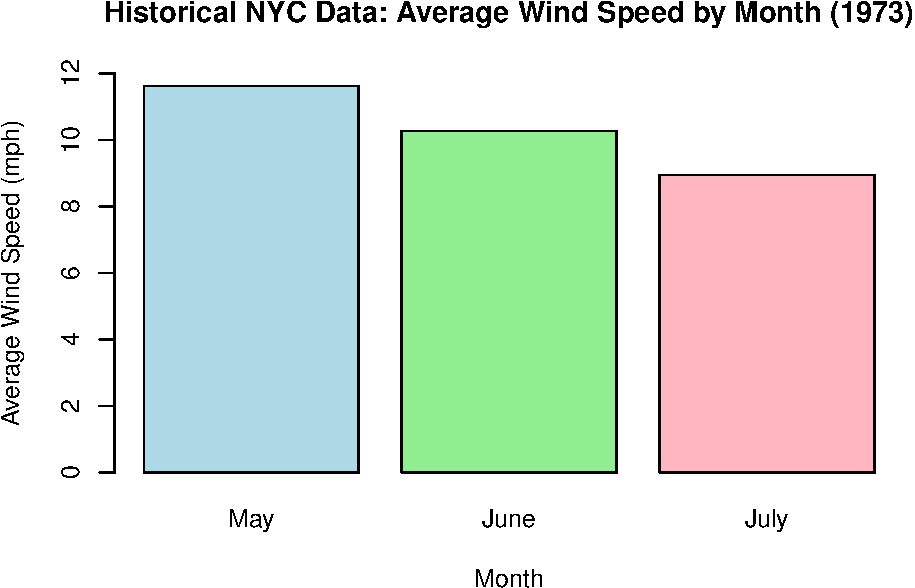
\includegraphics[keepaspectratio]{DataWranglingWithTidyverse_files/figure-latex/create_final_plot_revised-1.pdf}}

\subsection{Conclusion}\label{conclusion}

We have successfully completed our goal. We started with a messy,
report-style dataset and built a reproducible R script that transformed
it into a clean, tidy format. From this tidy data, we calculated a
summary statistic and created a clear visualization.

The key takeaway is that we now have a validated workflow. When we
receive our real air quality data from Williamsburg, we can confidently
adapt this script to quickly produce similar analyses. This is the power
of a well-designed data wrangling pipeline.

\section{A Quick Tour of Base R
Plots}\label{a-quick-tour-of-base-r-plots}

While ggplot2 is the modern standard, R's built-in plotting functions
are fast and great for quick exploratory work without loading any
additional libraries.

\subsection{Base R Plot: Scatterplot
(plot)}\label{base-r-plot-scatterplot-plot}

Purpose: To visualize the relationship between two continuous variables.

Example: Plot car weight vs.~miles per gallon from the built-in `mtcars'
dataset

\begin{Shaded}
\begin{Highlighting}[]
\FunctionTok{plot}\NormalTok{(mtcars}\SpecialCharTok{$}\NormalTok{wt, mtcars}\SpecialCharTok{$}\NormalTok{mpg,}
     \AttributeTok{main =} \StringTok{"Car Weight vs. MPG"}\NormalTok{,}
     \AttributeTok{xlab =} \StringTok{"Weight (1000 lbs)"}\NormalTok{,}
     \AttributeTok{ylab =} \StringTok{"Miles Per Gallon"}\NormalTok{,}
     \AttributeTok{pch =} \DecValTok{19}\NormalTok{) }\CommentTok{\# pch changes the point shape}
\end{Highlighting}
\end{Shaded}

\pandocbounded{
\includegraphics[keepaspectratio]{DataWranglingWithTidyverse_files/figure-latex/unnamed-chunk-3-1.pdf}}

\subsection{Base R Plot: Histogram
(hist)}\label{base-r-plot-histogram-hist}

Purpose: To understand the distribution of a single continuous variable.

Example: Plot the distribution of sepal lengths from the built-in `iris'
dataset

\begin{Shaded}
\begin{Highlighting}[]
\FunctionTok{hist}\NormalTok{(iris}\SpecialCharTok{$}\NormalTok{Sepal.Length,}
     \AttributeTok{main =} \StringTok{"Distribution of Sepal Lengths"}\NormalTok{,}
     \AttributeTok{xlab =} \StringTok{"Sepal Length"}\NormalTok{,}
     \AttributeTok{col =} \StringTok{"lightblue"}\NormalTok{) }\CommentTok{\# col sets the color}
\end{Highlighting}
\end{Shaded}

\pandocbounded{
\includegraphics[keepaspectratio]{DataWranglingWithTidyverse_files/figure-latex/unnamed-chunk-4-1.pdf}}

\subsection{Base R Plot: Bar Plot
(barplot)}\label{base-r-plot-bar-plot-barplot}

Purpose: To compare the size of different categories. Note: barplot
usually needs pre-summarized data (like averages across conditions).

\begin{Shaded}
\begin{Highlighting}[]
\CommentTok{\# First, create a summary table of counts for each cylinder type}
\NormalTok{cylinder\_counts }\OtherTok{\textless{}{-}} \FunctionTok{table}\NormalTok{(mtcars}\SpecialCharTok{$}\NormalTok{cyl)}

\CommentTok{\# Now, create the bar plot of the counts}
\FunctionTok{barplot}\NormalTok{(cylinder\_counts,}
        \AttributeTok{main =} \StringTok{"Number of Cars by Cylinder Type"}\NormalTok{,}
        \AttributeTok{xlab =} \StringTok{"Number of Cylinders"}\NormalTok{,}
        \AttributeTok{ylab =} \StringTok{"Count"}\NormalTok{,}
        \AttributeTok{col =} \FunctionTok{c}\NormalTok{(}\StringTok{"skyblue"}\NormalTok{, }\StringTok{"salmon"}\NormalTok{, }\StringTok{"lightgreen"}\NormalTok{))}
\end{Highlighting}
\end{Shaded}

\pandocbounded{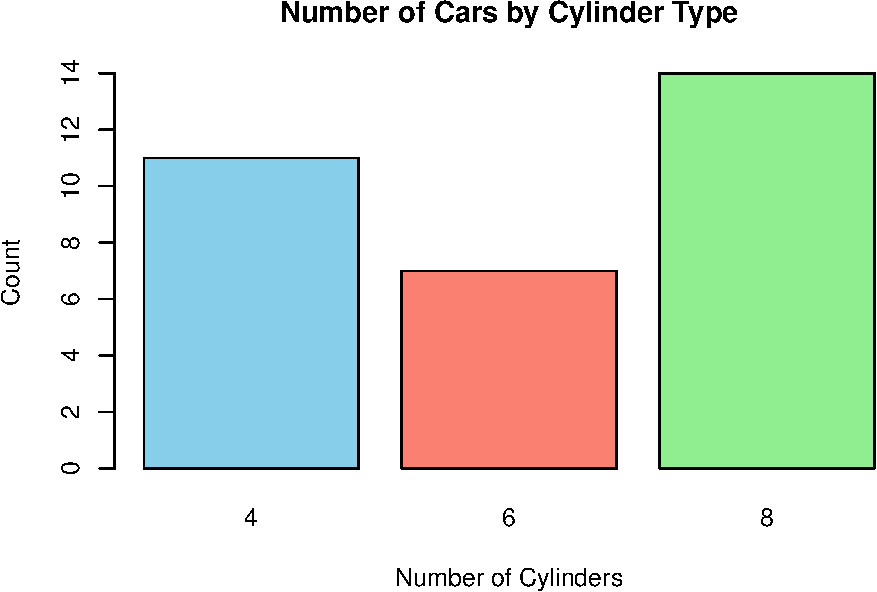
\includegraphics[keepaspectratio]{DataWranglingWithTidyverse_files/figure-latex/unnamed-chunk-5-1.pdf}}

\subsection{Base R Plot: Box Plot
(boxplot)}\label{base-r-plot-box-plot-boxplot}

Purpose: To compare the distribution of a continuous variable across
several groups.

Example: Compare MPG distribution for each cylinder type using formula
notation

\begin{Shaded}
\begin{Highlighting}[]
\FunctionTok{boxplot}\NormalTok{(mpg }\SpecialCharTok{\textasciitilde{}}\NormalTok{ cyl,}
        \AttributeTok{data =}\NormalTok{ mtcars,}
        \AttributeTok{main =} \StringTok{"MPG Distribution by Number of Cylinders"}\NormalTok{,}
        \AttributeTok{xlab =} \StringTok{"Number of Cylinders"}\NormalTok{,}
        \AttributeTok{ylab =} \StringTok{"Miles Per Gallon"}\NormalTok{,}
        \AttributeTok{col =} \StringTok{"skyblue"}\NormalTok{)}
\end{Highlighting}
\end{Shaded}

\pandocbounded{
\includegraphics[keepaspectratio]{DataWranglingWithTidyverse_files/figure-latex/unnamed-chunk-6-1.pdf}}

\section{Exercises}\label{exercises}

The following exercises will test your ability to apply the data
wrangling skills you've learned in this chapter. Each problem uses
datasets that are built into the Tidyverse, so you will need to have the
\texttt{tidyverse} library loaded. The goal is not just to get the right
answer, but to write a clean, readable pipeline of commands for each
task. \textbf{Don't forget to use text blocks and/or comments to
document your thinking and explain what each line of your code is
doing.}

\begin{Shaded}
\begin{Highlighting}[]
\FunctionTok{library}\NormalTok{(tidyverse)}
\end{Highlighting}
\end{Shaded}

\begin{center}\rule{0.5\linewidth}{0.5pt}\end{center}

\subsubsection{Problem 1: Analyzing US
Arrests}\label{problem-1-analyzing-us-arrests}

\textbf{Dataset:} \texttt{USArrests} (built into R)

\textbf{Scenario:} A law student at William \& Mary is researching
historical crime data from 1973 and wants to identify states with high
urban populations and their corresponding violent crime rates.

\textbf{Task:} Write a single pipeline of \texttt{dplyr} commands that:
1. Starts with the \texttt{USArrests} dataset. Note that the state names
are currently row names. You can turn them into a proper column by
running
\texttt{USArrests\ \%\textgreater{}\%\ rownames\_to\_column(var\ =\ "state")}
first. 2. Filters the data to include only states with an
\texttt{UrbanPop} rate of 80\% or higher. 3. Selects only the
\texttt{state}, \texttt{Murder}, and \texttt{Rape} columns. 4. Arranges
the final result by the \texttt{Murder} rate in descending order. 5.
Write a sentence or two to describe the result.

\begin{Shaded}
\begin{Highlighting}[]
\CommentTok{\# Your code here}
\end{Highlighting}
\end{Shaded}

\begin{center}\rule{0.5\linewidth}{0.5pt}\end{center}

\subsubsection{Problem 2: Mammal Sleep
Habits}\label{problem-2-mammal-sleep-habits}

\textbf{Dataset:} \texttt{msleep} (from the \texttt{ggplot2} package)

\textbf{Scenario:} A researcher at the Virginia Living Museum wants to
know if there's a relationship between an animal's diet and its sleep
patterns, specifically the proportion of time spent in REM sleep.

\textbf{Task:} Write a \texttt{dplyr} pipeline that: 1. Starts with the
\texttt{msleep} dataset. 2. Removes rows where the \texttt{vore} (diet)
column is \texttt{NA}, as we can't use them for this analysis. (Hint:
use \texttt{filter(!is.na(vore))}). 3. Creates a new column called
\texttt{rem\_proportion} which is the ratio of \texttt{sleep\_rem} to
\texttt{sleep\_total}. 4. Groups the data by \texttt{vore}. 5.
Calculates the average \texttt{rem\_proportion} for each diet group. 6.
Arranges the final tibble to show the diets with the highest average REM
proportion first. 7. Create a bar chart or boxplot to visualize the REM
proportion for each diet type. 8. Write a sentence or two to describe
the results.

\begin{Shaded}
\begin{Highlighting}[]
\CommentTok{\# Your code here}
\end{Highlighting}
\end{Shaded}

\begin{center}\rule{0.5\linewidth}{0.5pt}\end{center}

\subsubsection{Problem 3: Tidying Global Health
Data}\label{problem-3-tidying-global-health-data}

\textbf{Dataset:} \texttt{who} (from the \texttt{tidyr} package)

\textbf{Scenario:} An intern at the Virginia Department of Health has
been given a dataset from the World Health Organization about
tuberculosis cases. The data is in an extremely ``wide'' and messy
format and needs to be tidied before any analysis can be done.

\textbf{Task:} This is a classic reshaping challenge. The columns from
\texttt{new\_sp\_m014} through \texttt{newrel\_f65} contain values that
should be in their own columns. 1. Start with the \texttt{who} dataset.
2. Use \texttt{pivot\_longer()} to gather all the columns from
\texttt{new\_sp\_m014} to \texttt{newrel\_f65}. 3. The names of these
columns should go into a new column called \texttt{diagnosis\_code}. 4.
The values should go into a new column called \texttt{count}. 5. After
pivoting, many rows will have a \texttt{count} of \texttt{NA}. Filter
these rows out. 6. Display the first few rows of your final tidy tibble.

\emph{(Hint: This is a complex pivot! You can select the columns with
\texttt{cols\ =\ new\_sp\_m014:newrel\_f65})}

\begin{Shaded}
\begin{Highlighting}[]
\CommentTok{\# Your code here}
\end{Highlighting}
\end{Shaded}

\begin{center}\rule{0.5\linewidth}{0.5pt}\end{center}

\subsubsection{Problem 4: Finding the Windiest Year for
Storms}\label{problem-4-finding-the-windiest-year-for-storms}

\textbf{Dataset:} \texttt{storms} (from the \texttt{dplyr} package)

\textbf{Scenario:} Meteorologists in Hampton Roads are analyzing the
historical Atlantic storm dataset to identify the year with the highest
average maximum wind speeds, which could indicate a particularly active
storm season.

\textbf{Task:} Write a \texttt{dplyr} pipeline to determine which year
had the highest average wind speeds for its storms. Your final output
should be a tibble with only one row (the winning year). 1. Start with
the \texttt{storms} dataset. 2. Group the data by \texttt{year}. 3. For
each year, calculate the average maximum wind speed (\texttt{wind}). 4.
Arrange the results to find the year with the highest average. 5. Create
a scatter plot of year as a function of wind speed. 6. Return only the
top row. (Hint: \texttt{head(1)} or \texttt{slice\_max()} are good ways
to do this). 7. Write a sentence or two to describe your results.

\begin{Shaded}
\begin{Highlighting}[]
\CommentTok{\# Your code here}
\end{Highlighting}
\end{Shaded}

\begin{center}\rule{0.5\linewidth}{0.5pt}\end{center}

\subsubsection{Problem 5: From Tidy back to
Wide}\label{problem-5-from-tidy-back-to-wide}

\textbf{Dataset:} Your tidied data from Problem 3.

\textbf{Scenario:} After you tidied the \texttt{who} dataset, your
manager asks for a specific summary table: a report showing the total
number of cases for Afghanistan, Brazil, and China for the years 1999
through 2001. They want the years as columns for a quick comparison.

\textbf{Task:} This requires you to filter, summarize, and then reshape
your tidy data back into a wide format. 1. Start with the tidied data
you created in Problem 3. 2. \texttt{filter()} for only the countries of
interest (\texttt{Afghanistan}, \texttt{Brazil}, \texttt{China}) and the
years of interest (\texttt{1999}, \texttt{2000}, \texttt{2001}). 3.
Calculate the total number of cases (\texttt{count}) for each country
and year combination. (Hint: \texttt{group\_by()} then
\texttt{summarise()}). 4. Use \texttt{pivot\_wider()} to reshape this
summary table. The new column headers should come from the \texttt{year}
column, and the values should come from your new \texttt{total\_cases}
column. 5. Write a sentence or two to describe your results.

\begin{Shaded}
\begin{Highlighting}[]
\CommentTok{\# First, re{-}create your tidy \textquotesingle{}who\textquotesingle{} data from problem 3 here}
\CommentTok{\# tidy\_who \textless{}{-} who \%\textgreater{}\% ...}

\CommentTok{\# Then, write the pipeline for this problem}
\CommentTok{\# tidy\_who \%\textgreater{}\% ...}
\end{Highlighting}
\end{Shaded}

\subsubsection{Problem 6: Ranking Species by Average BMI (Star
Wars)}\label{problem-6-ranking-species-by-average-bmi-star-wars}

\textbf{Dataset:} starwars (from dplyr)

\textbf{Scenario:} A sci‑fi physiology class wants to compare species by
average Body Mass Index (BMI), computed from height and mass.

\subsubsection{Task:}\label{task}

Write a pipeline that:

\begin{enumerate}
\def\labelenumi{\arabic{enumi}.}
\item
  Starts from starwars, and keeps name, species, height, mass.
\item
  Creates height\_m = height / 100 and bmi = mass / (height\_m\^{}2).
\item
  Groups by species, computes avg\_bmi and n (characters per species).
\item
  Ungroup and return the top 5 species by avg\_bmi, breaking ties by n
  (larger first).
\item
  Create a visualization (plot) of your results.
\item
  Write a sentence or two to describe your results.
\end{enumerate}

(Tip: This reinforces mutate(), summarise(), arrange(), and the
importance of ungroup().)

\begin{Shaded}
\begin{Highlighting}[]
\CommentTok{\# Your code here}
\end{Highlighting}
\end{Shaded}

\subsubsection{\texorpdfstring{Problem 7: Advanced Reshaping with
\texttt{.value} (Water
Quality)}{Problem 7: Advanced Reshaping with .value (Water Quality)}}\label{problem-7-advanced-reshaping-with-.value-water-quality}

\textbf{Dataset:} Recreate the \texttt{water\_quality\_wide} tibble from
the chapter (or copy it in your chunk).

\textbf{Scenario:} You need a tidy table that separates pollutant and
statistic, then a compact report.

\textbf{Task:}\\
1. Start from \texttt{water\_quality\_wide} (columns like
\texttt{nitrogen\_mean}, \texttt{nitrogen\_sd}, etc.).

\begin{enumerate}
\def\labelenumi{\arabic{enumi}.}
\setcounter{enumi}{1}
\item
  Use \texttt{pivot\_longer()} with
  \texttt{names\_to\ =\ c("pollutant",\ ".value")} and
  \texttt{names\_sep\ =\ "\_"} to get columns
  \texttt{site,\ collection\_date,\ pollutant,\ mean,\ sd}.
\item
  Compute \textbf{overall means by pollutant} (average of the
  \texttt{mean} column across sites/dates).
\item
  Return a \textbf{one‑row per pollutant} report and then
  \texttt{pivot\_wider()} so pollutants are columns and the overall
  means are values.
\item
  Write a sentence or two describing your results.
\end{enumerate}

\emph{(Tip: This exercises the advanced \texttt{.value} pattern and a
round‑trip pivot.)}

\begin{Shaded}
\begin{Highlighting}[]
\CommentTok{\# Your code here}
\end{Highlighting}
\end{Shaded}


\bibliography{Introduction2R.bib}

\end{document}
